\documentclass[a4paper, 12pt]{article}%twoside,
\usepackage{amssymb}
\usepackage{amsmath}
\allowdisplaybreaks[1] %如果用align之類的東西,東西太長時,不會整段換頁
\usepackage{xeCJK}
\usepackage{ragged2e}
%%%\usepackage{CJK}Microsoft JhengHei UI
\setCJKmainfont{cwTeXFangSong}
%{微軟正黑體}%{仿宋體}%{標楷體}
\XeTeXlinebreaklocale "zh"
\XeTeXlinebreakskip = 0pt plus 1pt %這兩行一定要加,中文才能自動換行

%AMS 數學環境
\usepackage{amsmath}
\usepackage{amssymb}
\usepackage{amsthm}
\usepackage{relsize}
\usepackage{mathtools} %新一代數學工具,修正一點amsmath的bug

\usepackage{xcolor}
\usepackage{array}
%圖片
\usepackage{graphicx}  %插入图片的宏包
\usepackage{float}     %设置图片浮动位置的宏包
\usepackage{subfigure} %插入多图时用子图显示的宏包

 %% font & format %%
\usepackage[margin=2cm]{geometry} % 上下左右距離邊緣2cm

\usepackage{type1cm}	% 設定fontsize用
\usepackage{titlesec}   % 設定section等的字體
\usepackage{fancyhdr}   % 頁首頁尾
\usepackage{multicol}   % 多欄 \multicols
\usepackage{ulem}       % 字加裝飾 (underline+emphasis)(我不會用)

\usepackage{yhmath}     % BIG math symbol,如matrix用的超大圓括弧、角括弧
\usepackage{tikz-cd}    % 含tikz,可以多畫diagram類的東西
\usepackage{diagbox}    % 可以在表格畫斜線
% \usepackage{caption}
% \usepackage{subcaption}

    
    %% Enhancement %%
\usepackage{titling}    % 加強 title 功能
\usepackage{tabularx}   % 加強版 table
\usepackage{booktabs}   % toprule, bottomrule...
\usepackage{enumerate}   % 加強版enumerate, itemize, list
\usepackage[showzone=true, showseconds=true]{datetime2} %加強版時間格式
\usepackage[square, comma, numbers, super, sort&compress]{natbib}  % cite加強版

\usepackage{wasysym}    % 可以打出各種怪符號如 \sun, \smiley, \eighthnote
\usepackage{dsfont}     % 另一種雙標線字體 \mathds,多了\mathds{1 h k}
\usepackage[scr]{rsfso} % 草寫字體 \mathscr,請只使用其中一個
%\usepackage{BOONDOX-uprscr} % 另一個草寫字體 \mathscr,請只使用其中一個

\usepackage{bigints} % 大積分
\usepackage{extarrows} % 長等號
\usepackage{multirow} % 表格多列合併
\renewcommand\arraystretch{1.2}

\theoremstyle{definition}
\newtheorem*{theorem}{Theorem}
\newtheorem{thm}{Theorem}
\newtheorem*{df}{Definition}
\newtheorem{ex}[thm]{Example}
\newtheorem{exs}[thm]{Exercise}
\newtheorem*{cl}{Corollary}
\newtheorem{pp}[thm]{Property}
\newtheorem*{prop}{Proposition}
\newtheorem*{lm}{Lemma}
\newtheorem{pr}{Problem}
\newtheorem*{ft}{Fact}
\newtheorem{note}{Note}[pr]
\newtheorem*{hint}{Hint}
\renewcommand{\proofname}{\bf Proof:\\} %修改Proof 標頭,Proof有內建
\newtheorem*{rec}{Recall}
\newtheorem*{pf}{Proof}
\newenvironment{subpf}{{\small \textbf{subproof.} }}{\hfill {\small \qedsymbol{}}}
\newtheorem*{rmk}{Remark}
\newtheorem*{clm}{Claim}
\newtheorem{sol}{Solution}
\newtheorem*{ins}{Instance}
\newtheorem{inst}{Instance}

%定義一些符號command:
\newcommand{\N}{\mathbb{N}}
\newcommand{\Z}{\mathbb{Z}}
\newcommand{\Q}{\mathbb{Q}}
\newcommand{\R}{\mathbb{R}}
\newcommand{\C}{\mathbb{C}}
\newcommand{\E}{\mathbb{E}}
\renewcommand{\P}{\mathbb{P}}

\newcommand{\be}{\begin{equation}}
\newcommand{\ee}{\end{equation}}
\newcommand{\bear}{\begin{eqnarray*}}
\newcommand{\eear}{\end{eqnarray*}}
\newcommand{\bearr}{\begin{eqnarray}}
\newcommand{\eearr}{\end{eqnarray}}
\newcommand{\bi}{\begin{itemize}}
\newcommand{\ei}{\end{itemize}}
\newcommand{\bn}{\begin{enumerate}}
\newcommand{\en}{\end{enumerate}}
\newcommand{\bd}{\begin{description}}%\bd[]
\newcommand{\ed}{\end{description}}
\newcommand{\I}{\item}
\newcommand{\varep}{\varepsilon}
\newcommand{\mc}[1]{{\mathcal #1}}
\newcommand{\mf}[1]{{\mathfrak #1}}
\newcommand{\mb}[1]{{\mathbf #1}}
\newcommand{\bb}[1]{{\mathbb #1}}
\newcommand{\lf}{\left}
\newcommand{\rt}{\right}
\newcommand{\st}{\mbox{ s.t }}
\newcommand{\ti}{\textit}
\newcommand{\p}[1]{\phantom{#1}}
\newcommand{\pa}{\phantom{a}}
\newcommand{\ans}{\medskip{\bf Ans.}}
% \newcommand{\hl}[1]{\colorbox{yellow}{#1}}
\renewcommand{\note}[1]{{\bf Note #1.}}
\usepackage{authblk}

\usepackage{caption}
\usepackage{subcaption}

%==================================================================%

%\pagestyle{empty} %後的指令不會執行(ignored),可供撰寫comment
\setlength{\textwidth}{18.5cm}
\setlength{\oddsidemargin}{-1.7cm}
\setlength{\evensidemargin}{1pt}
\setlength{\topmargin}{-3cm}
\setlength{\textheight}{26.5cm}
\setlength{\droptitle}{-2cm} 

% \geometry{bottom=3cm}
\geometry{a4paper,left=3cm,right=3cm,top=3cm,bottom=3cm} 
% \usepackage{pgfplots}
% \pgfplotsset{compat=1.5}

% \title{\textbf{Operations Research Final Project}\\
\title{Operations Research Final Project\\
Optimal Planning for NTU YouBike Assignment}

% \title{\sc{Operations Research}\\\large{Final Project}\\Optimal Planning for 
% NTU YouBike Assignment }
\author{
Group A\\
吳驊祐\, B09705009 \ 周成康\, B09705011 \ 陳瑾叡\, B09705016\qquad\qquad 黃戎僔\, B09705032 \ 吳天冷\, B08303135 \ 李詠如\, B07703084\qquad\qquad 劉德駿\, B07801013 \ 李宗霖\, B07702044 \ 陳琳瑄\, B06B02059\qquad\qquad}
\date{June 10, 2022}

\begin{document}
\maketitle
\justifying


\section{Introduction}

% \hspace*{0.7cm}

Many of us might have the following experience. After a tiring day at school, you plan to ride a YouBike to have a nice meal, however, there is no available YouBike in the station. After a long wait, you finally get a YouBike and arrive at the restaurant, you realize that there is no empty dock to return it. YouBike is supposed to be a convenience transportation option for citizens. However, such situation happens every day, and is kind of annoying.\\

\noindent This problem is due to the \hl{\textbf{imbalanced demand distributions}}, which is related to our daily routine. For example, on weekday mornings, students ride YouBikes from MRT stations and dormitories to teaching buildings. We can observe that some stations receive YouBikes more than providing to others and some stations provide YouBikes more than receiving from others; therefore, YouBikes keep being accumulated in those "receiving-stations", while those "providing-stations" are consistently under-supplied. Although we often see the trucks shuttling back and forth in campus, working hard on repositioning YouBikes, the severe spatial imbalance still exists. Around NTU, there are \hl{\textbf{102 stations and 1800 docks}} in total. During peak time, more than 300 YouBikes are needed to be repositioned while a truck can only ship 16 bikes at most. What's more, if we take a look at both large stations and small stations, $30\%$ and $80\%$ of docks are vacant, respectively. With the evidence mentioned above, this is indeed a problematic issue in urgent need of being solved.\\

\noindent Even though this kind of imbalance is inevitable and could not be entirely eliminated, the operators should minimize it, otherwise it could cause negative effects on revenue. Due to the reasons mentioned above, we decided to take a deep look into the issue, to see if we could figure out a better way to reposition YouBikes. There are only two options available, either the operators move YouBikes by themselves, or they provide customers incentives to do it for them (e.g., price discounts \footnote{https://www.iot.gov.tw/dl-11486-61bf1c0d3d214be0b7800566fa19921d.html}).\\

\noindent In this project, we choose the former way and focus on the stations in NTU District. Although we focus on NTU District only, the same concept can be applied in any area. After all, to minimize the cost and maximize the efficiency, a single truck should not be in charge of a wide area. Suppose that the YouBike company decide to rent trucks for repositioning YouBikes and reschedule the routes. Our goal is to generate an optimal route that minimizes the cost and balances the percentage of available YouBikes in each station at the same time.

% \subsection{Motivation}

% As a NTU student, one might have been in a situation where he/she cannot gain access to bike-sharing service, \hl{\textbf{YouBike}}, when he/she was in urgent need. 

% \noindent Observing this kind of phenomena, we can't help but being curious about \emph{How} the bikes are dispatched behind the secret of YouBike service and \emph{why} sometimes one can barely fulfill his/her demand for the prevalent bike-sharing service.

% \subsection{Evidence}

% To illustrate, a series of evidences that indicates how challenging and necessary the YouBike assignment issue is are provided.
%\begin{enumerate}
    %\item The Expected bike capacity to meet minimum demand at GongGuan station in peak time slots are around \hl{\textbf{300-400}} bikes.
    %\item The capacity of a general truck are only around \hl{\textbf{16}} bikes.
    %\item Less then \hl{\textbf{30\%}} of large stations (having more than 25 docks) are having less than \emph{5} bikes available in peaked time slots. On the other hand, Less then \hl{\textbf{80\%}} of small stations (having less than 15 docks) are having less than \emph{5} bikes available in peaked time slots. 
%\end{enumerate}


\section{Problem Description}

Our goal is to minimize the total cost and all possible negative impact, i.e., shortage and surplus that this dispatching problem may incur. This problem can be considered as a vehicle routing problem, which is NP-hard, and hence it is arduous to solve. \\ \\
% \subsection{Sets}
\noindent Interestingly, for this problem can be solved successfully, two virtual points are needed. Index $0$ and index $N+1$ both stand for virtual points, which are labeled as "Start" and "End", respectively.

\subsection{Decision Variables}

% There are 10 decision variables in this problem, and they are as follows.

\subsubsection{Major Variables}

The following variables are involved in the objective function, which means the objective value is determined by them.
% \begin{enumerate}
%     \item $y_{ij} = 1$ if the truck moves from station $i$ to $j$ and $0$ otherwise, $y_{ij} \in \{0,1\}$
%     \item $w_{iL}$: The percentage shortage after dispatching of station $i$
%     \item $w_{iH}$: The percentage surplus after dispatching of station $i$
% \end{enumerate}

    \begin{table}[h!]
        \centering
        \begin{tabular}{l|l}
    	\toprule
           $y_{ij}$ &1  if the truck moves from station $i$ to $j$ and $0$ otherwise, $y_{ij} \in \{0,1\}$ \\ \hline
           $w_{iL}$ &  The percentage shortage after dispatching of station $i$, $w_{iL} \geq 0$ \\
            $w_{iH}$& The percentage surplus after dispatching of station $i$, $w_{iH} \geq 0$ \\
    	\bottomrule
        \end{tabular}
        \caption{Major Decision Variables}
        \label{tab:my_labe1l}
    \end{table}

\noindent Among all the major variables above, the $y_{ij}$'s are used for cost calculation. The $w_{iL}$'s and $w_{iH}$'s are related to penalty, if shortage and surplus happen to exist, i.e., the acceptable parking ratio is failed to be achieved, there should be sanctions imposed on the objective value.

% $y_{ij} = 1$ if the truck moves from station $i$ to $j$ and $0$ otherwise, $y_{ij} \in \{0,1\}$ \\
% $w_{iL}$: The percentage shortage after dispatching of station $i$\\
% $w_{iH}$: The percentage surplus after dispatching of station $i$\\


\subsubsection{Derived Variables}
While the major variables directly determine the objective value, the derived variables are essential for constraints.

\newpage

% \begin{enumerate}
%     \item $x_i = 1$ if station $i$ visited by the truck and $0$ otherwise, $x_i \in \{0,1\}$
%     \item $a_i$: The number of bikes taken away from station $i$, $a_i \geq 0$
%     \item $b_i$: The number of bikes dispatched to station $i$, $b_i \geq 0$
%     \item $p_i$: The number of bikes on a truck when arriving at station $i$, $p_i \geq 0$
%     \item $q_i$: The number of bikes on a truck when leaving station $i$, $q_i \geq 0$
%     \item $u_i$: The order (number) in a truck's tour of station $i$, $u_i \geq 0$
%     \item $v_{ij} = 1$ if station $i$ is visited later than station $j$ and 0 otherwise, $v_{ij} \in \{0,1\}$
% \end{enumerate}


    \begin{table}[h!]
        \centering
        \begin{tabular}{c|l}
    	\toprule
           $x_i$ & 1 if station $i$ visited by the truck and $0$ otherwise, $x_i \in \{0,1\}$\\ \hline 
            $a_i$ & The number of bikes taken away from station $i$, $a_i \geq 0$\\
            $b_i$ &  The number of bikes dispatched to station $i$, $b_i \geq 0$\\
            $p_i$ &  The number of bikes on a truck when arriving at station $i$, $p_i \geq 0$\\
            $q_i$ & The number of bikes on a truck when leaving station $i$, $q_i \geq 0$\\ \hline
            $u_i$ & The order (number) in a truck's tour of station $i$, $u_i \geq 0$\\ 
            $v_{ij}$  & 1 if station $i$ is visited later than station $j$ and 0 otherwise, $v_{ij} \in \{0,1\}$\\
    	\bottomrule
        \end{tabular}
        \caption{Derived Decision Variables}
        \label{tab:my_labe1l}
    \end{table}


\noindent Among all the derived variables above, the $x_i$'s are crucial for restricting the $y_{ij}$'s. The $a_i$'s, $b_i$'s, $p_i$'s and $q_i$'s are required for the determination of the $w_{iL}$'s and $w_{iH}$'s. The $u_i$'s and $v_{ij}$'s are critical for subtour elimination. 


% \newpage
\subsection{Parameters}

% There are 12 parameters in this problem, and they are listed below.


\begin{table}[h!]
    \centering
    \begin{tabular}{cl}
	\toprule
        \multicolumn{2}{c}{{\textbf{Parameters Concerning Trucks and Bikes}}}  \\ \hline
        $C_{ij}$ & The distance of a truck moving from station $i$ to $j$\\
        & (Let $C_{00}  = C_{N+1,0} = C_{N+1,N+1} = 0$,   $C_{0,N+1} = - T/G $.) \\
        $Parked_i$ & The number of bikes parked at station $i$ at the moment \\
        $Capacity_i$ & The capacity of station $i$ \\
        $M$ & The sum of parked bikes \\
        $G$ & The gas price per kilometer \\
        $T$ & The cost of renting a truck \\ \hline
        \multicolumn{2}{c}{{\textbf{Parameters Concerning Limitations}}} \\ \hline
        $A$& The maximum capacity of a truck used for dispatching \\
        $L$& The maximum distance for a truck to move \\ \hline
        \multicolumn{2}{c}{{\textbf{Parameters Concerning Penalty}}} \\ \hline
        $S_L$ &  Lower bound of acceptable parking ratio\\
        $S_H$ &  Upper bound of acceptable parking ratio\\
        $\lambda$& The coefficient for penalty arising from shortage or surplus in dispatching\\ \hline
        \multicolumn{2}{c}{{\textbf{Parameters Concerning Subtours}}} \\ \hline
        $e$ &  The constant for ensuring the relationship between the $u_{ij}$'s (orders).\\
	\bottomrule
    \end{tabular}
    \caption{Parameters}
    \label{tab:Parameters}
\end{table}


% \begin{enumerate}
%     \item $C_{ij}$: The distance of a truck moving from station $i$ to $j$\\ (Let $C_{00} = C_{0,N+1} = C_{N+1,0} = C_{N+1,N+1} < 0 $.)
%     \item $Parked_i$: The number of bikes parked at station $i$ at the moment
%     \item $Capacity_i$: The capacity of station $i$
%     \item $M$: The sum of parked bikes
%     \item $G$: The gas price per kilometer
%     \item $T$: The cost of renting a truck
% \end{enumerate} 



% \subsubsection{Parameters Concerning Limitations}
% \begin{enumerate}
%     \item $A$: The maximum capacity of a truck used for dispatching
%     \item $L$: The maximum distance for a truck to move
% \end{enumerate}


% \subsubsection{Parameters Concerning Penalty}
% \begin{enumerate}
%     \item $S_L$: Lower bound of acceptable parking ratio
%     \item $S_H$: Upper bound of acceptable parking ratio
%     \item $\lambda$: The coefficient for penalty arising from shortage or surplus in dispatching
% \end{enumerate}

\noindent It is worthwhile to notice that the $S_L$ and $S_H$ provide bounds for acceptable parking ratio so that an interval can be formed. The size of the interval should be correlated with $\lambda$, for the interval's size can be thought of as the "elasticity" for parking; different degrees of penalty should be granted to different elasticity.
Therefore, we set the interval's size as the following.
\[[0.5 - \lambda, 0.5 + \lambda]\]
Note that the size of the interval is positively correlated with $\lambda$, in other words, larger interval implies that it is more inelastic to the number of bike changes and severer penalty should be meted out for not achieving the acceptable parking ratio.

% \subsubsection{Parameters Concerning Subtours}
% \begin{enumerate}
%     \item $e$: The constant for ensuring the relationship between the $u_{ij}$'s (orders).
% \end{enumerate}


% The Parameters included



\subsection{Objective Function and Constraints}

After defining our parameters and variables, the complete formulation can be constructed as the following.
    
\subsubsection{Objective Function}

\noindent The function can be split into three parts. The first term denotes the cost total cost of dispatching (traveling through stations); the second term represents the penalty associated with shortage and surplus, and the last term is the cost of renting a truck.
\begin{align}
    \min \quad G \sum_{i = 0}^{N+1} \sum_{j = 0}^{N+1} y_{ij} C_{ij} + \lambda (100 \sum_{i = 1}^N (w_{iL} + w_{iH}))^2 + T
\end{align}

\subsubsection{Constraints for Routing}

\noindent For the sake of moving from one station to another, both stations must be visited. 
\begin{align}
    \quad  x_i + x_j \geq 2(y_{ij} + y_{ji}), \quad  \forall i, j = 0,...,N+1
\end{align}

\noindent For each station, arrival implies departure, and vice versa.
\begin{align}
    \quad  \sum_{i = 0}^N y_{ik} = \sum_{i = 1}^{N+1} y_{kj}, \quad  \forall k = 1,...,N
\end{align}

\noindent It is not reasonable for a truck to move from a station to the same one.
\begin{align}
    \quad  y_{ij} = 0, \quad  \forall i,j = 0,...,N+1, i = j
\end{align}

\noindent A truck cannot move back to the previous station.
\begin{align}
    \quad  y_{ij} + y_{ji} \leq 1, \quad  \forall i, j = 0,...,N+1
\end{align}

\noindent A truck cannot move for more than the maximum distance.
\begin{align}
    \quad  \sum_{i = 0}^{N+1} \sum_{j = 0}^{N+1} C_{ij} y_{ij} \leq L
\end{align}

\noindent A truck can only arrive at and leave a station once.
\begin{align}
    \quad  \sum_{i = 0}^{N+1} y_{ij} \leq 1, \quad  \forall j = 0,...,N+1 \\
    \quad \sum_{j = 0}^{N+1} y_{ij} \leq 1, \quad  \forall i = 0,...,N+1
\end{align}

\noindent A visit of a station implies the arrival at it and / or the departure from it.
\begin{align}
    \quad  \sum_{j = 0}^{N+1} y_{ij} + \sum_{j = 0}^{N+1} y_{ji} \geq x_i, \quad  \forall i = 0,...,N+1
\end{align}

\subsubsection{Constraints for Bikes}
\noindent Do not take away bikes and dispatch bikes at the same time.
\begin{align}
    \quad  a_i b_i = 0, \quad  \forall i = 0,...,N+1
\end{align}

\noindent Take away / Dispatch bikes only if a station is visited.
\begin{align}
    \quad  a_i \leq M x_i, \quad  \forall i = 0,...,N+1 \\
    \quad  b_i \leq M x_i, \quad \forall i = 0,...,N+1
\end{align}

\noindent Penalize when there is shortage or surplus. 
\begin{align}
    \quad  & w_{iL} \geq S_L - \frac{Parked_i - a_i + b_i}{Capacity_i}, \quad  \forall i = 1,...,N \\
    \quad  & w_{iL} \geq 0, \quad  \forall i = 1,...,N \\
    \quad  & w_{iH} \geq \frac{Parked_i - a_i + b_i}{Capacity_i} - S_H, \quad  \forall i = 1,...,N \\
    \quad  & w_{iH} \geq 0, \quad  \forall i = 1,...,N
\end{align}

\noindent The flow-in must be equivalent to the flow-out for each station. 
\begin{align}
    \quad  \sum_{i = 0}^{N+1} a_i x_i = \sum_{i = 0}^{N+1} b_i x_i
\end{align}

\noindent Dispatch bikes to a station reasonably. 
\begin{align}
    \quad  b_i + Parked_i \leq Capacity_i, \quad  \forall i = 1,...,N+1
\end{align}

\noindent Take away bikes from a station reasonably.
\begin{align}
    \quad  a_i \leq Parked_i, \quad  \forall i = 1,...,N
\end{align}

\subsubsection{Constraints for Trucks}

\noindent When a truck visit a station, bikes are either taken away from or dispatched to it. The following equation describes the change in the number of bikes on a truck. 
\begin{align}
    \quad p_i + a_i - b_i = q_i, \quad \forall i = 0,...,N+1
\end{align}

\noindent The number of bikes on a truck when leaving a station must equal to that when arriving at the next one. 
\begin{align}
    \quad q_i y_{ij} = p_j y_{ij}, \quad \forall i,j = 0,...,N+1
\end{align}

\noindent The number of bikes on a truck cannot exceed the maximum capacity of it. 
\begin{align}
    \quad p_i \leq A, q_i \leq A, \quad \forall i = 0,...,N+1
\end{align}

\noindent The number of bikes dispatched to a station cannot be greater than that on a truck when arriving. 
\begin{align}
    \quad b_i \leq p_i, \quad \forall i = 0,...,N+1
\end{align}

\subsubsection{Constraints for Virtual Points}

\noindent No bikes are taken away from and dispatched to Start. 
\begin{align}
    \quad a_0 = 0, b_0 = 0
\end{align}

\noindent No bikes are taken away from End, while it is acceptable to be dispatched to it. 
\begin{align}
    \quad a_{N+1} = 0, b_{N+1} \geq 0
\end{align}

\noindent A truck must visit Start and End. 
\begin{align}
    \quad x_0 = 1, x_{N+1} = 1
\end{align}

\noindent No arrival at Start, and no departure from End. 
\begin{align}
    \quad y_{i0} = 0, \quad \forall i = 1,...,N+1 \\
    \quad y_{N+1,i} = 0, \quad \forall i = 0,...,N
\end{align}

\noindent No bikes are on a truck at Start, and no bikes are leaving End. However, when arriving at End, the presence of bikes is acceptable. 
\begin{align}
    \quad & p_0 = 0, q_0 = 0 \\
    \quad & p_{N+1} \geq 0, q_{N+1} = 0
\end{align}

\noindent No penalty for Start and End. 
\begin{align}
    \quad & w_{0L} = 0, w_{0H} = 0 \\
    \quad & w_{N+1,L} = 0, w_{N+1,H} = 0
\end{align}

\subsubsection{Constraints for Eliminating Subtours}

\noindent In order to deal with subtours, the following constraints are indispensable.
\begin{align}
\quad &  u_0 = 1  & \\
\quad & u_i \leq N+2, \quad  &  \forall i = 1,...,N+1  \\
\quad &  u_i \geq 2, \quad  &  \forall i = 1,...,N+1 \\
\quad &  u_i - u_j + 1 \leq M(1 - y_{ij}), \quad  &  \forall i,j = 0,...,N+1, i \neq j \\
\quad &  u_i - u_j \leq M v_{ij} - e, \quad  &  \forall i,j = 0,...,N+1, i \neq j \\
\quad &  u_i - u_j \geq e - M(1 - v_{ij}), \quad   & \forall i,j = 0,...,N+1, i \neq j
\end{align}

\subsubsection{Sign Constraints}
\begin{align}
    \quad & y_{ij} \in \{0,1\}, \quad  & \forall i,j = 0,...,N+1 \\
    \quad & w_{iL} \geq 0, w_{iH} \geq 0, \quad  & \forall i = 0,...,N+1 \\
    \quad & x_i \in \{0,1\}, \quad  & \forall i = 0,...,N+1 \\
    \quad & a_i \geq 0, b_i \geq 0, p_i \geq 0, q_i \geq 0, \quad  & \forall i = 0,...,N+1 \\
    \quad & u_i \geq 0, v_{ij} \in \{0,1\}, \quad  & \forall i,j = 0,...,N+1
\end{align}


\noindent The complete formulation is
\[\begin{split}
  \min \ & (1) \\
  \mbox{s.t.} & (2)--(43).
\end{split}\]


% \[\begin{split}
%   \min \ & (\ref{eq:obj}) \\
%   \mbox{s.t.} & (\ref{eq:con_first})--(\ref{eq:con_last}).
% \end{split}\]

\section{Data Collection}
The data is from Open Government Data Platform, which is a platform operated by National Development Council. The data are obtained by web crawling and then organized into the format shown as below. \\

\begin{figure}[hbt]
    \centering
    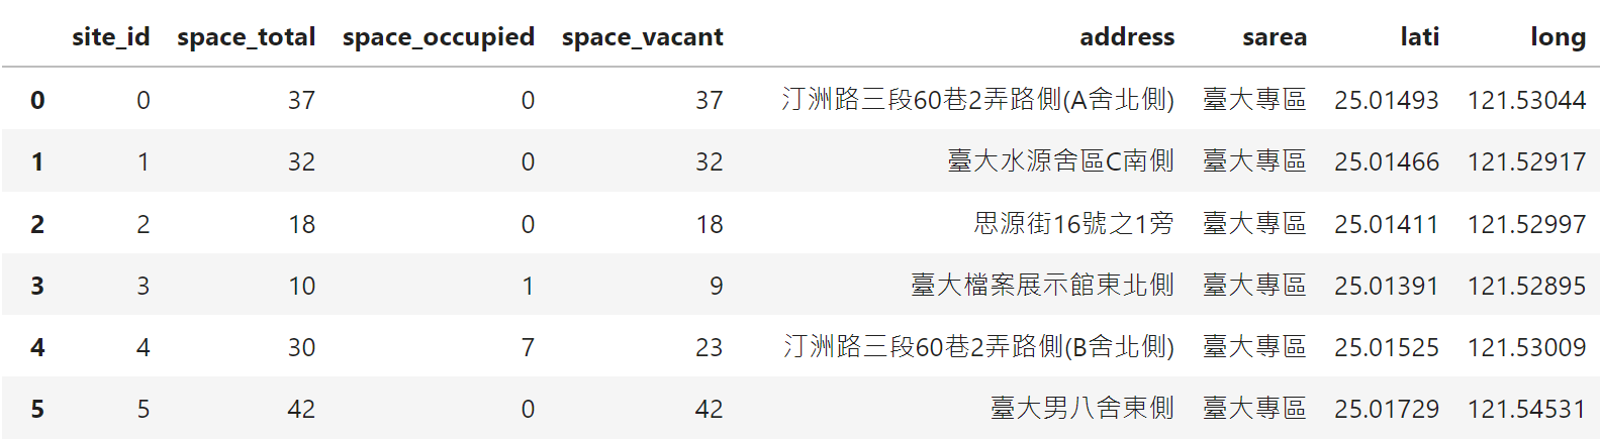
\includegraphics[width=0.7\textwidth]{Final/fig/data.png}
    \caption{The Organized Data of YouBike 2.0}
    \label{fig:data}
\end{figure}



\noindent The latitude and longitude are used for calculating the distances among the stations with the haversine formula. However, using such method for distance calculation is evidently unrealistic in our research; therefore, Google Application Programming Interface (API) is applied instead so that distances for trucks to move can be calculated accurately. 

\section{Method}
\noindent Our strategy is comprised of four procedures, which are \hl{\textbf{clustering, optimization, visualization, and analysis.}} \\

\noindent First of all, $k \verb|-means|$ clustering algorithm is implemented for the purpose of dividing stations into several clusters, i.e., $k$ groups. The clustering is based on the latitude-longitude coordinate system. \\

\noindent After that, different values of $k$ and $\lambda$ are chosen for invoking the \hl{\textbf{Gurobi solver}} to optimize our problem, and thus different objective values with different combinations of $k$ and $\lambda$ are pinned down. \\

\noindent Consequently, different objective values reported by Gurobi are visualized so as to determine which combination of the two parameters to choose under a certain circumstance. \\

\noindent Lastly, the results acquired with the chosen pair of $k$ and $\lambda$ are further analyzed for our truck routing problem.



\section{Results}

% 我們使用許多不同時間點測試模型的可行性,以下舉兩個例子解釋我們最後挑選參數的方法與決策機制。
\noindent We have tested our model with different data in different time to check feasibility. The following two instances demonstrate how the parameters are determined. 

\subsection{Instance 1: 6/1 17:00}

% 圖二為在不同分群的k與不同lambda組合下,模型算出的objective value,從中可以發現當lambda越大時,objective value 的值越低。有些分群結果為infeasible,表示在該群數下有至少一個子群超過時間限制。因此不列入選擇範圍中。

% 在此四種lambda條件下,如果以成本因素為主要考量,我們會選擇objective value最低的$\lambda = 0.35$ and $k = 2$作為決策的參數設定。

% 當確定$\lambda$ 與 分群數之後,模型將會給出站點調度的路線圖(如圖三),並會告訴調度員從哪個站點出發,與在該站點是執行拿車還是取車。在調度前的車輛分佈如圖4,其中有部分紅色的站點表示目前的車輛數低於$S_L$,藍色的站點則高於$S_H$。在經過調度後的結果如圖五,可以發現原本低於$S_L$的紅色站點數量下降,高於$S_H$的藍色站點數量也下降。即表示在經過調度後,原本缺車的站點有被補足,原本較多車的站點也有將車子移至需要車的站點。


\begin{figure}[hbt]
    \centering
    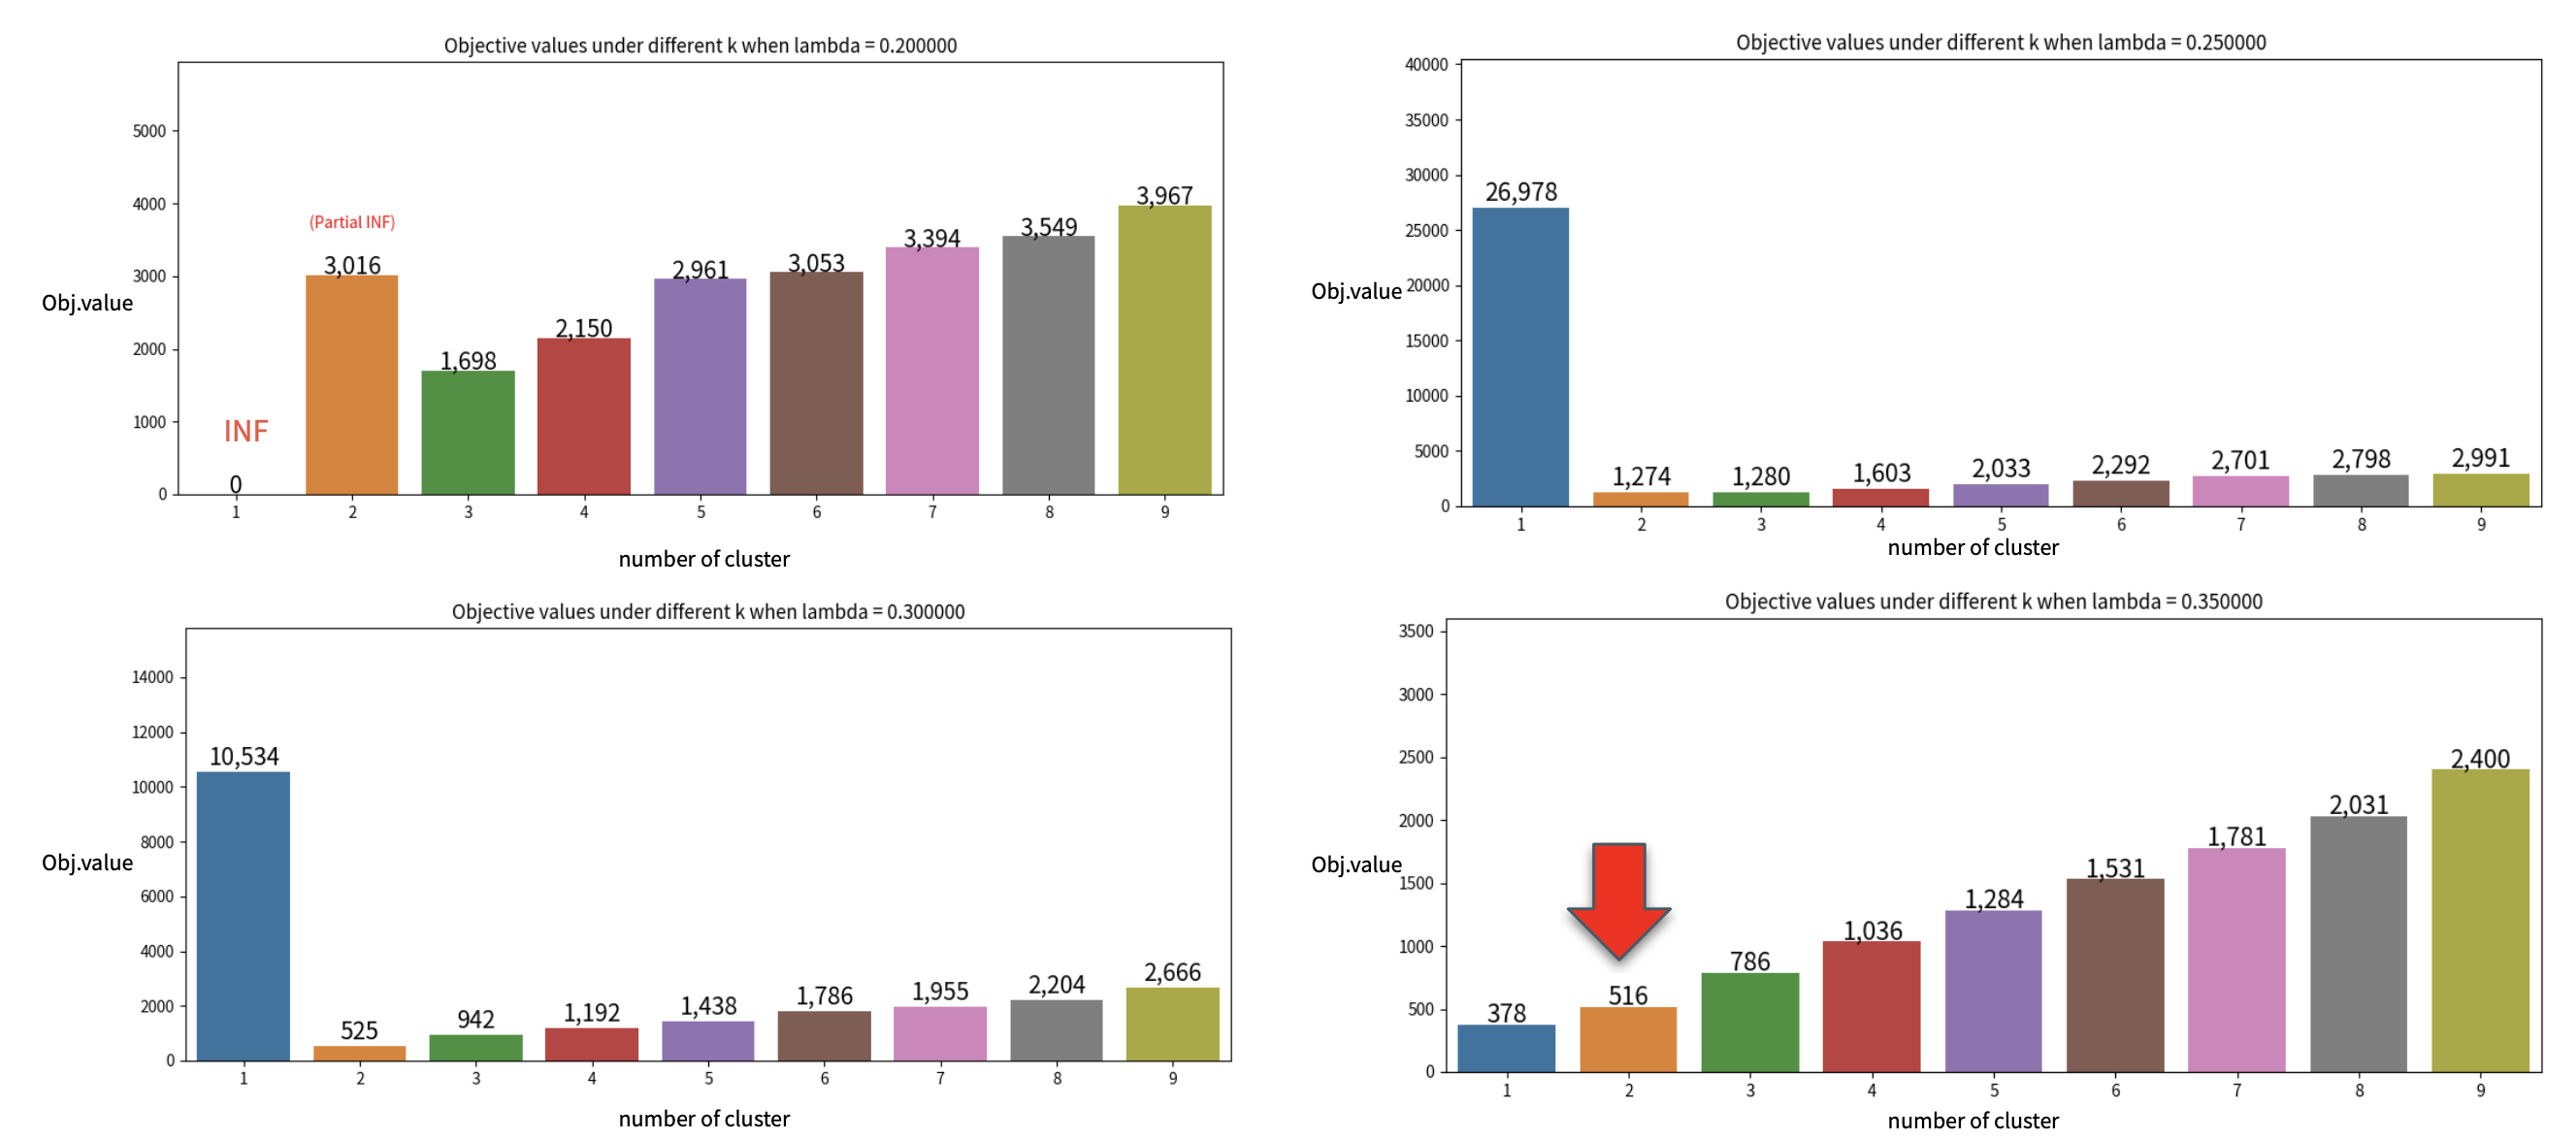
\includegraphics[width=0.8\textwidth]{Final/fig/bar_1.png}
    \caption{Objective Values under Different $\lambda$s and Clusters in Instance 1}
    \label{fig:bar-1}
\end{figure}

\noindent Figure \ref{fig:bar-1} shows different objective values generated with different combinations of $k$s and $\lambda$s. It is evident that larger $\lambda$  leads to smaller objective value. Also note that some of the results in clustering is infeasible, where at least one group does not satisfy the time constraint, and therefore not considered in our decision making.\\ 

\noindent Given these four lambdas, if cost is our main consideration in decision making, the smallest $\lambda$ and $k$, which are 0.35 and 2 respectively, would be chosen as our settings in parameters.\\


\noindent After $\lambda$ and $k$ are pinned down, our model would suggest routes for dispatching in figure \ref{fig:1-map}. The model would also indicate where to start our assignment and either to take away bikes from or to dispatch them to a station. Before the assignment, the distribution of bikes is depicted as figure \ref{fig:1-before}, where red spots denote the stations whose parking ratio lies beneath $S_L$ while the blue ones represent the opposite, i.e., their parking ratios exceed $S_H$. After the assignment, we can see the results as figure \ref{fig:2-after} illustrates. It is apparent that either the number of red spots or that of blue spots decreases, which means that we have successfully move bikes to those stations that are under supplied and move out bikes from the over supplied.

\begin{figure}[hbt]
    \centering
    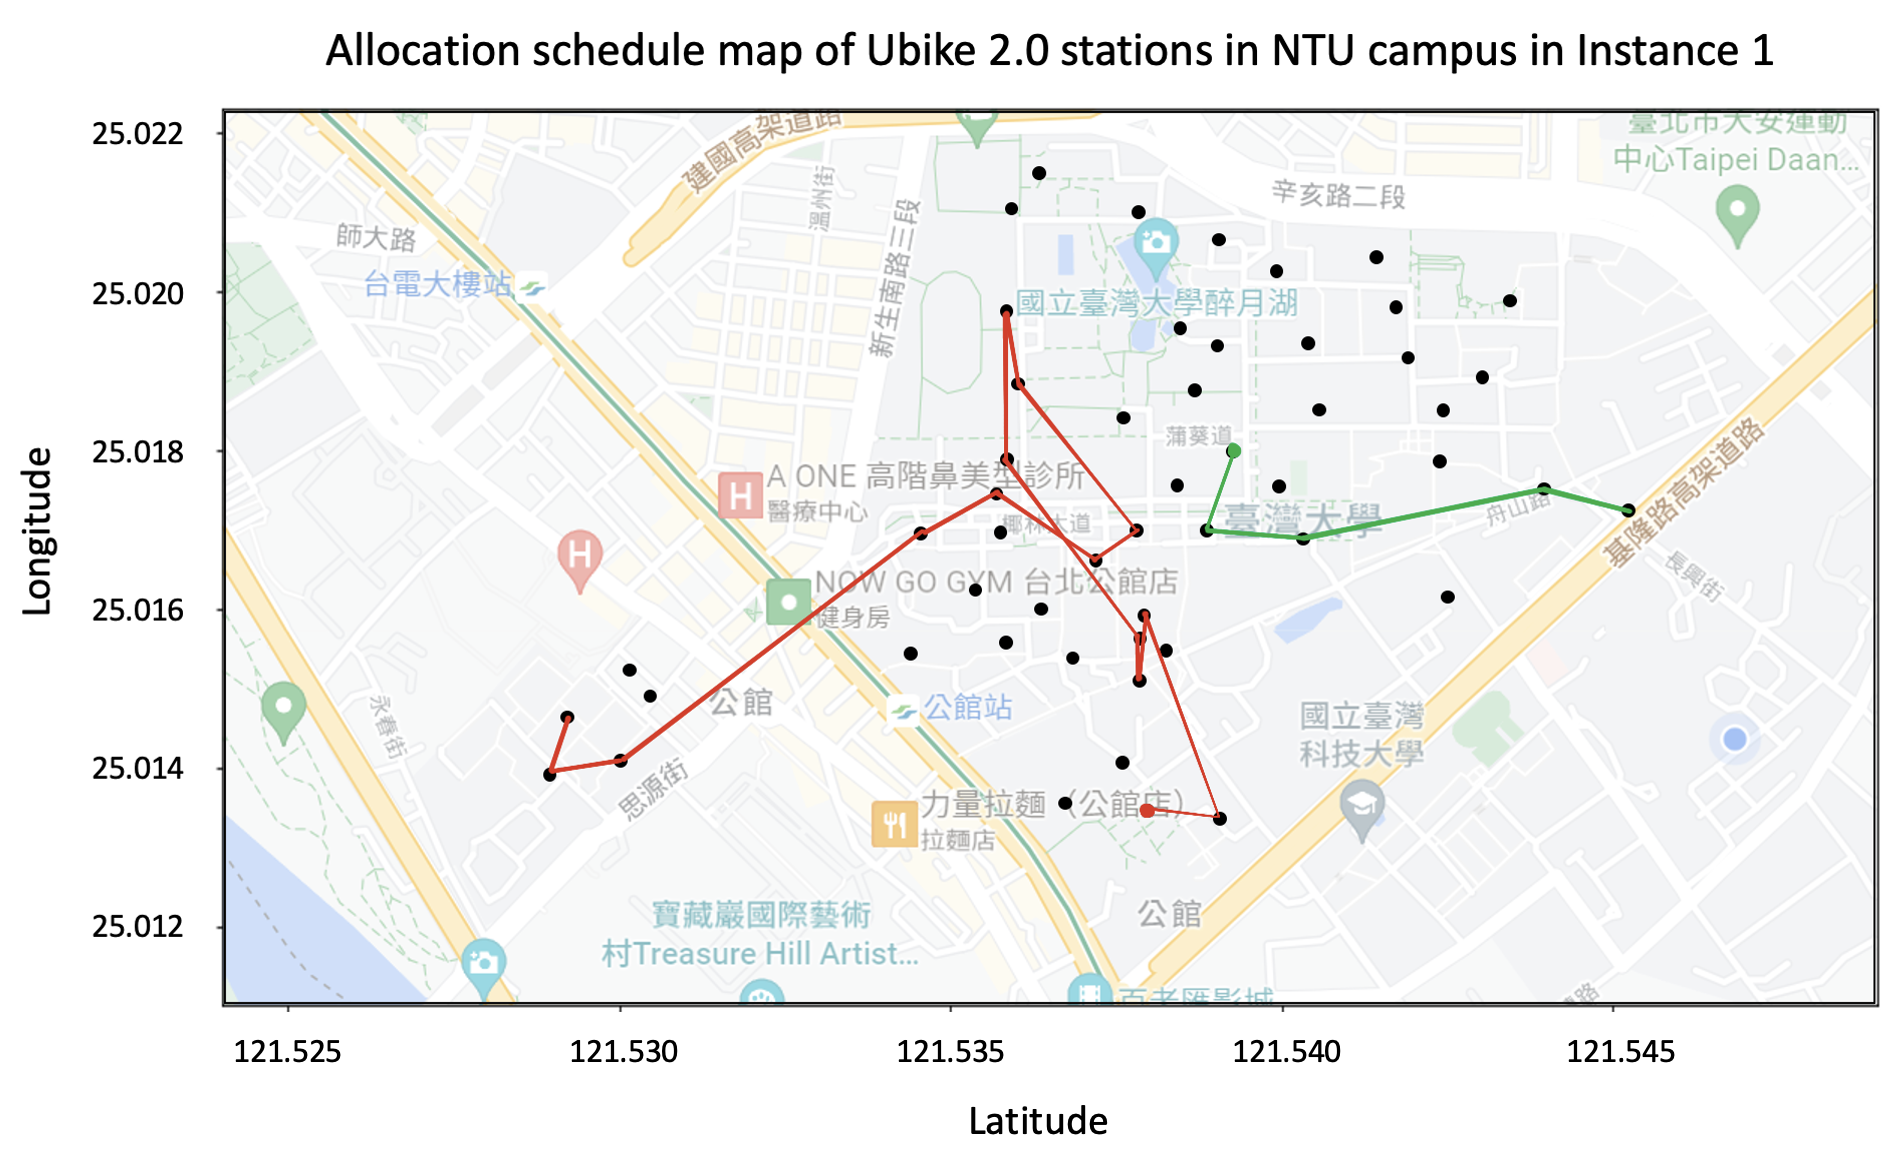
\includegraphics[width=0.9\textwidth]{Final/fig/Map1.png}
    \caption{The Allocation Schedule Map in Instance 1}
    \label{fig:1-map}
\end{figure}


\begin{figure}[hbt]
\centering
	\begin{minipage}[b]{0.45\textwidth}
		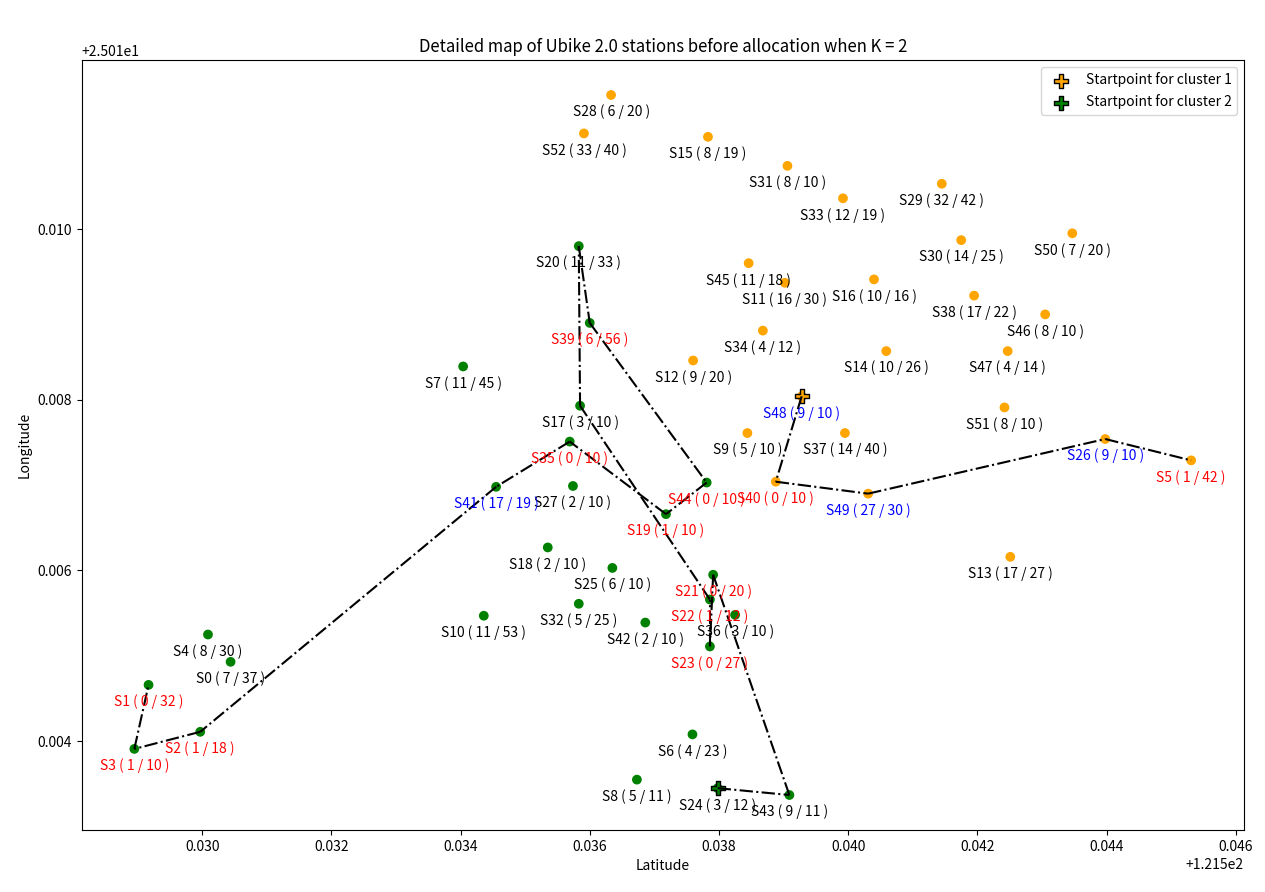
\includegraphics[width=\textwidth]{Final/fig/c1/4-2-4_Before Allocation Map.png}
		\caption{Detailed Ratio of YouBike Before Allocation in Instance 1}
		\label{fig:1-before}
	\end{minipage}
	\begin{minipage}[b]{0.05\textwidth}
		\quad
	\end{minipage}	
	\begin{minipage}[b]{0.45\textwidth}
		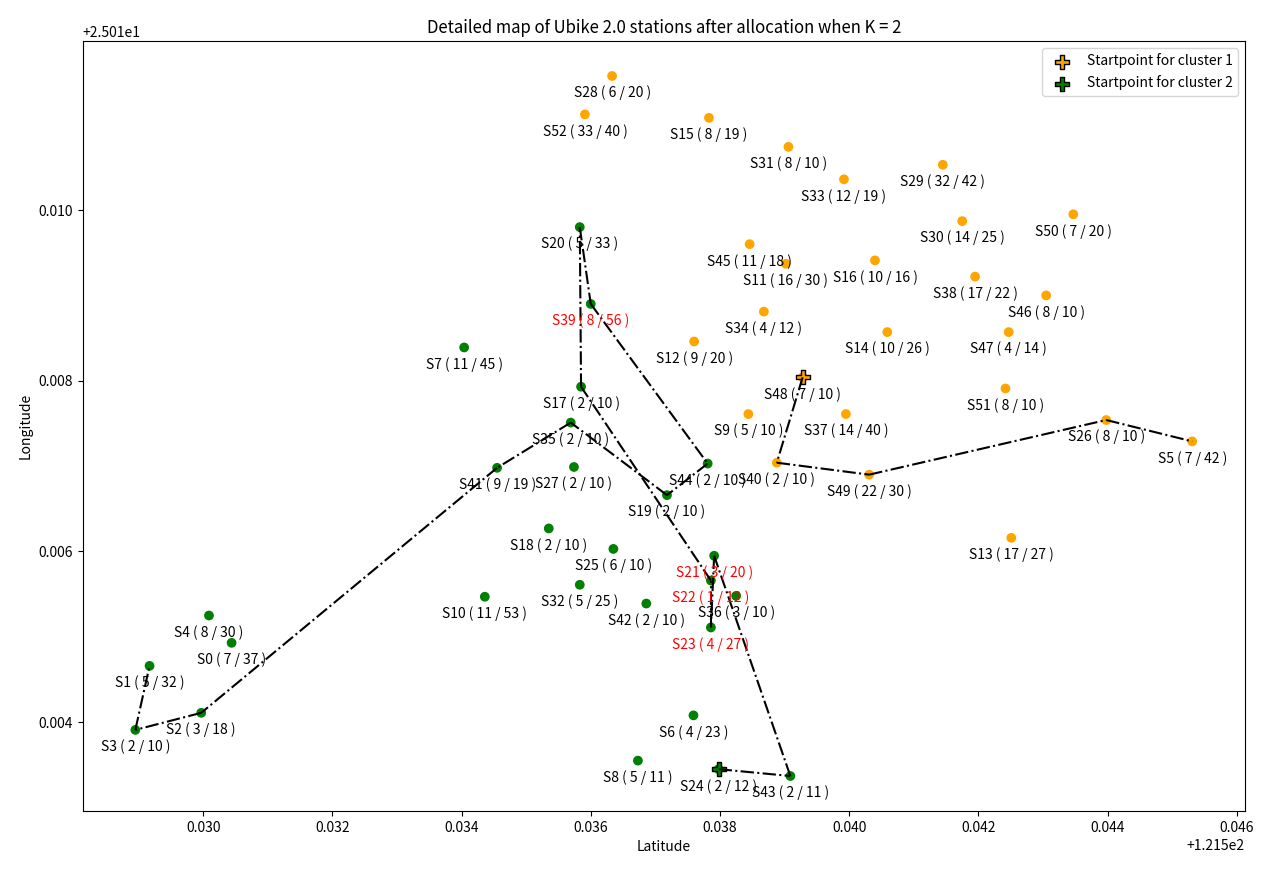
\includegraphics[width=\textwidth]{Final/fig/c1/4-2-3_After Allocation Map.png}
		\caption{Detailed Ratio of YouBike After Allocation in Instance 1}
		\label{fig:1-after}
	\end{minipage}
\end{figure}




\subsection{Instance 2: 6/3 8:00}

% 依照同樣的邏輯,先由不同組合的lambda與分群數跑出目標值(如圖六),再進一步挑選合適的參數。這次是在lambda=0.35 且分群數為8的條件下,跑出了最低的目標值。

% 圖七為分成8群的搬動路線圖,左下角的那群為不需出動調度車搬移的case。在調度前(圖八),我們可以看到大部分的站點都是較缺乏車輛的紅色站點,在經過調度後(如圖九)紅色站點的數量雖有減少,但還是有部分存在。我們推論是因為本時段本身在區域內的腳踏車供給數較低,因此就算出動較多台車,仍無法將所有站點都調度至合適的區間範圍內。

\noindent By same logic, that is, derive objective values under different combinations of $\lambda$ and $k$s and then choose the appropriate pair of the parameters (as shown in figure 6). This time, $\lambda$ is 0.35 and $k$ is 8.

\begin{figure}[hbt]
    \centering
    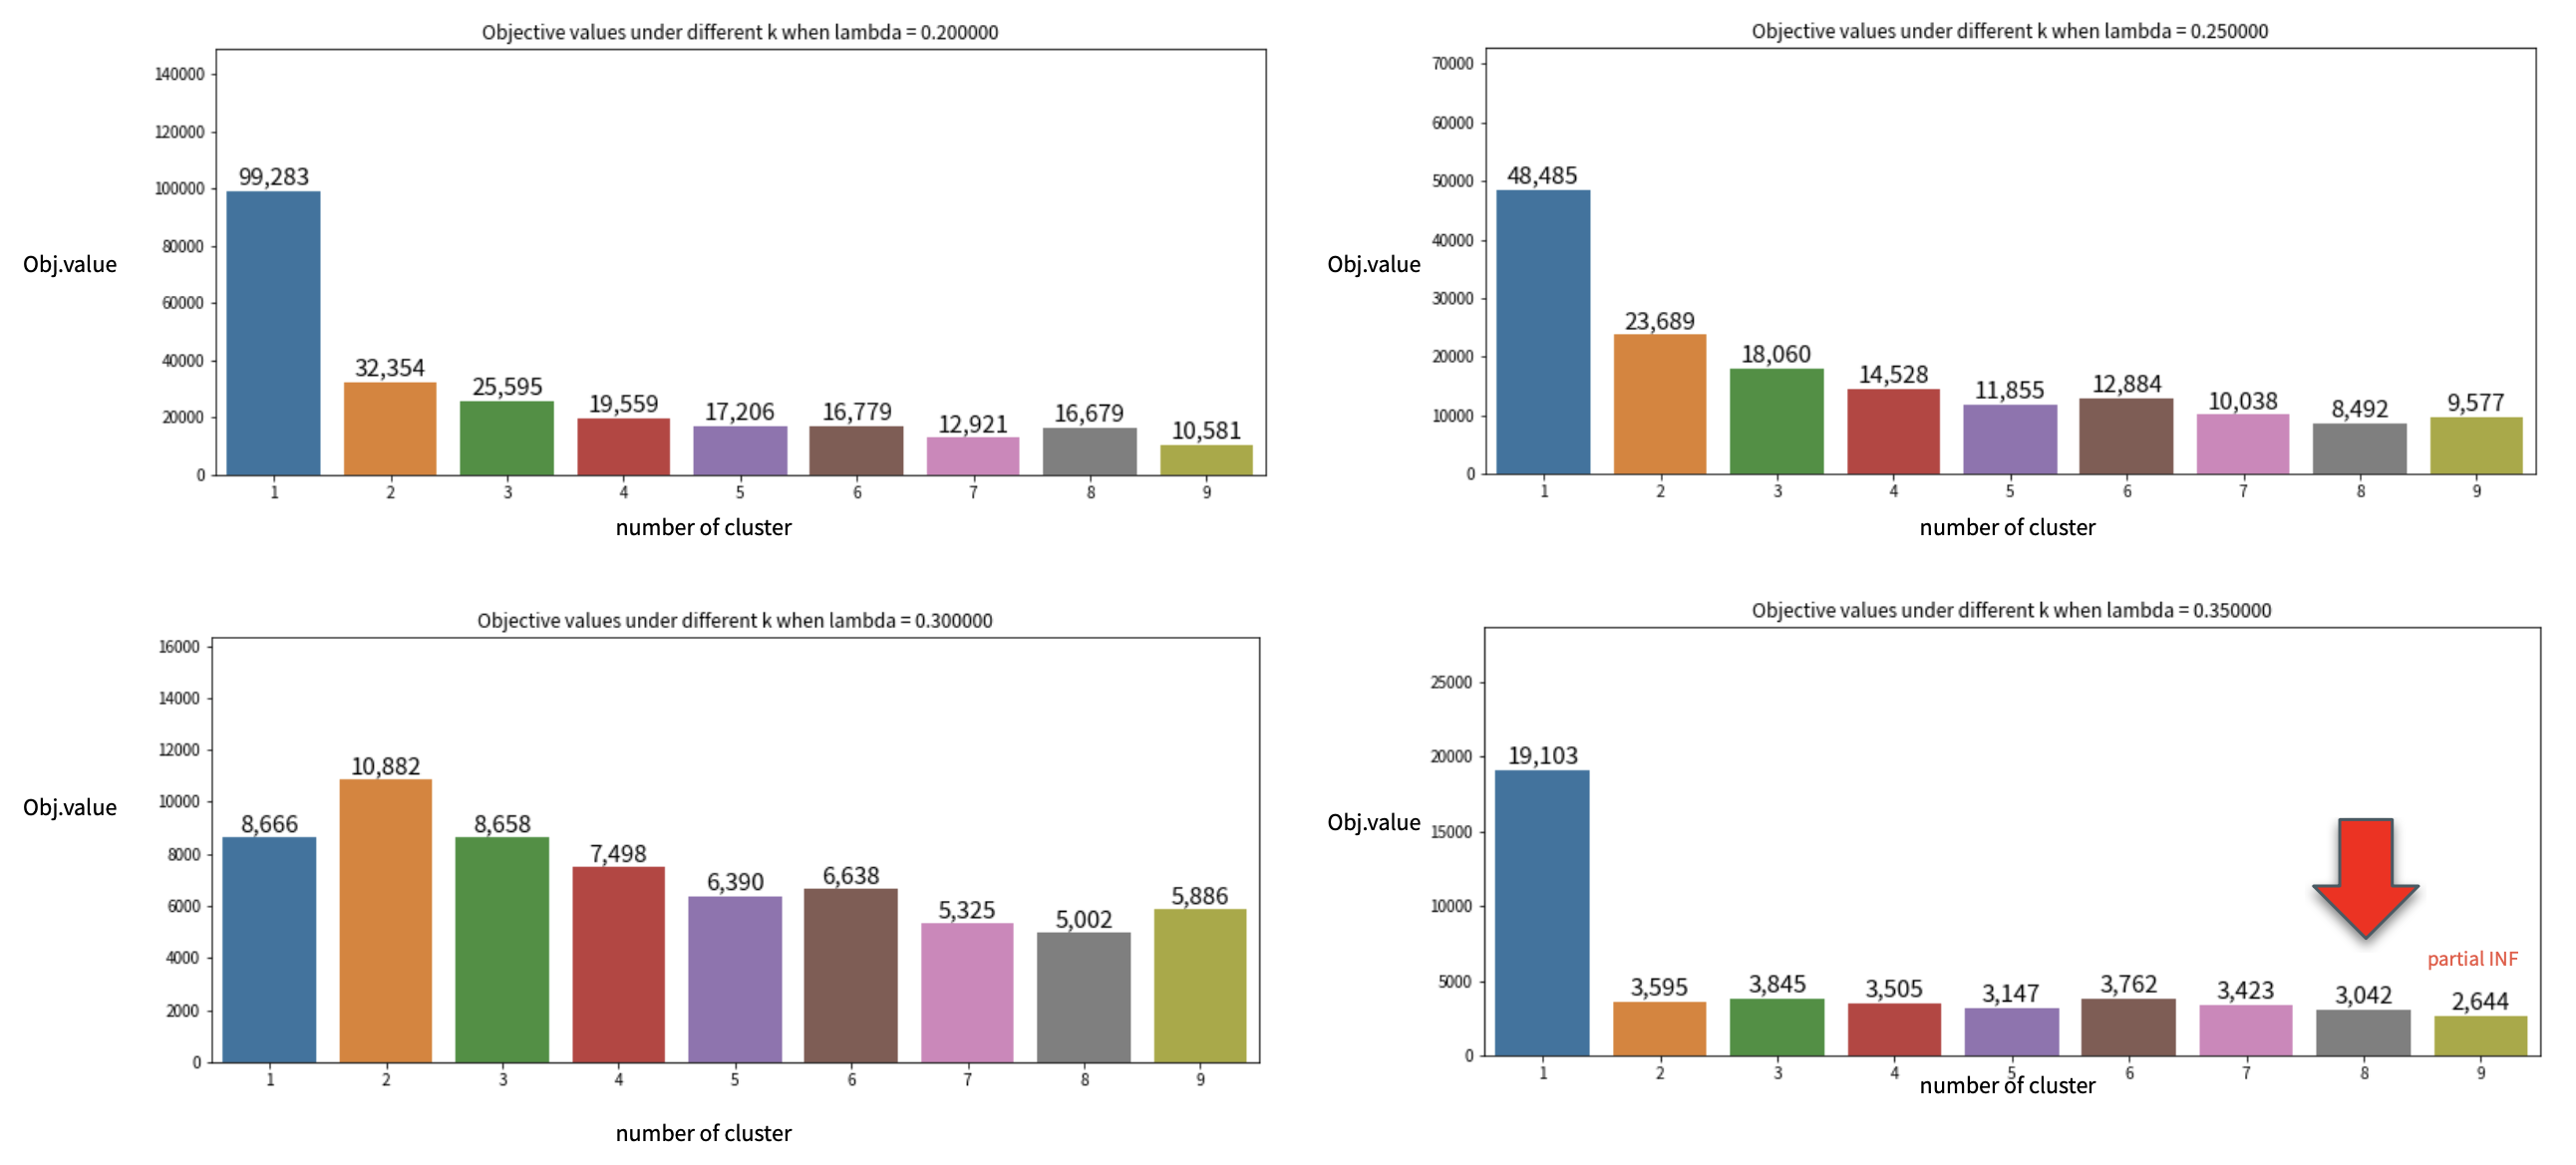
\includegraphics[width=0.8\textwidth]{Final/fig/bar_2.png}
    \caption{Objective Values under Different $\lambda$s and Clusters in Instance 2}
    \label{fig:bar-2}
\end{figure}
\begin{figure}[hbt]
    \centering
    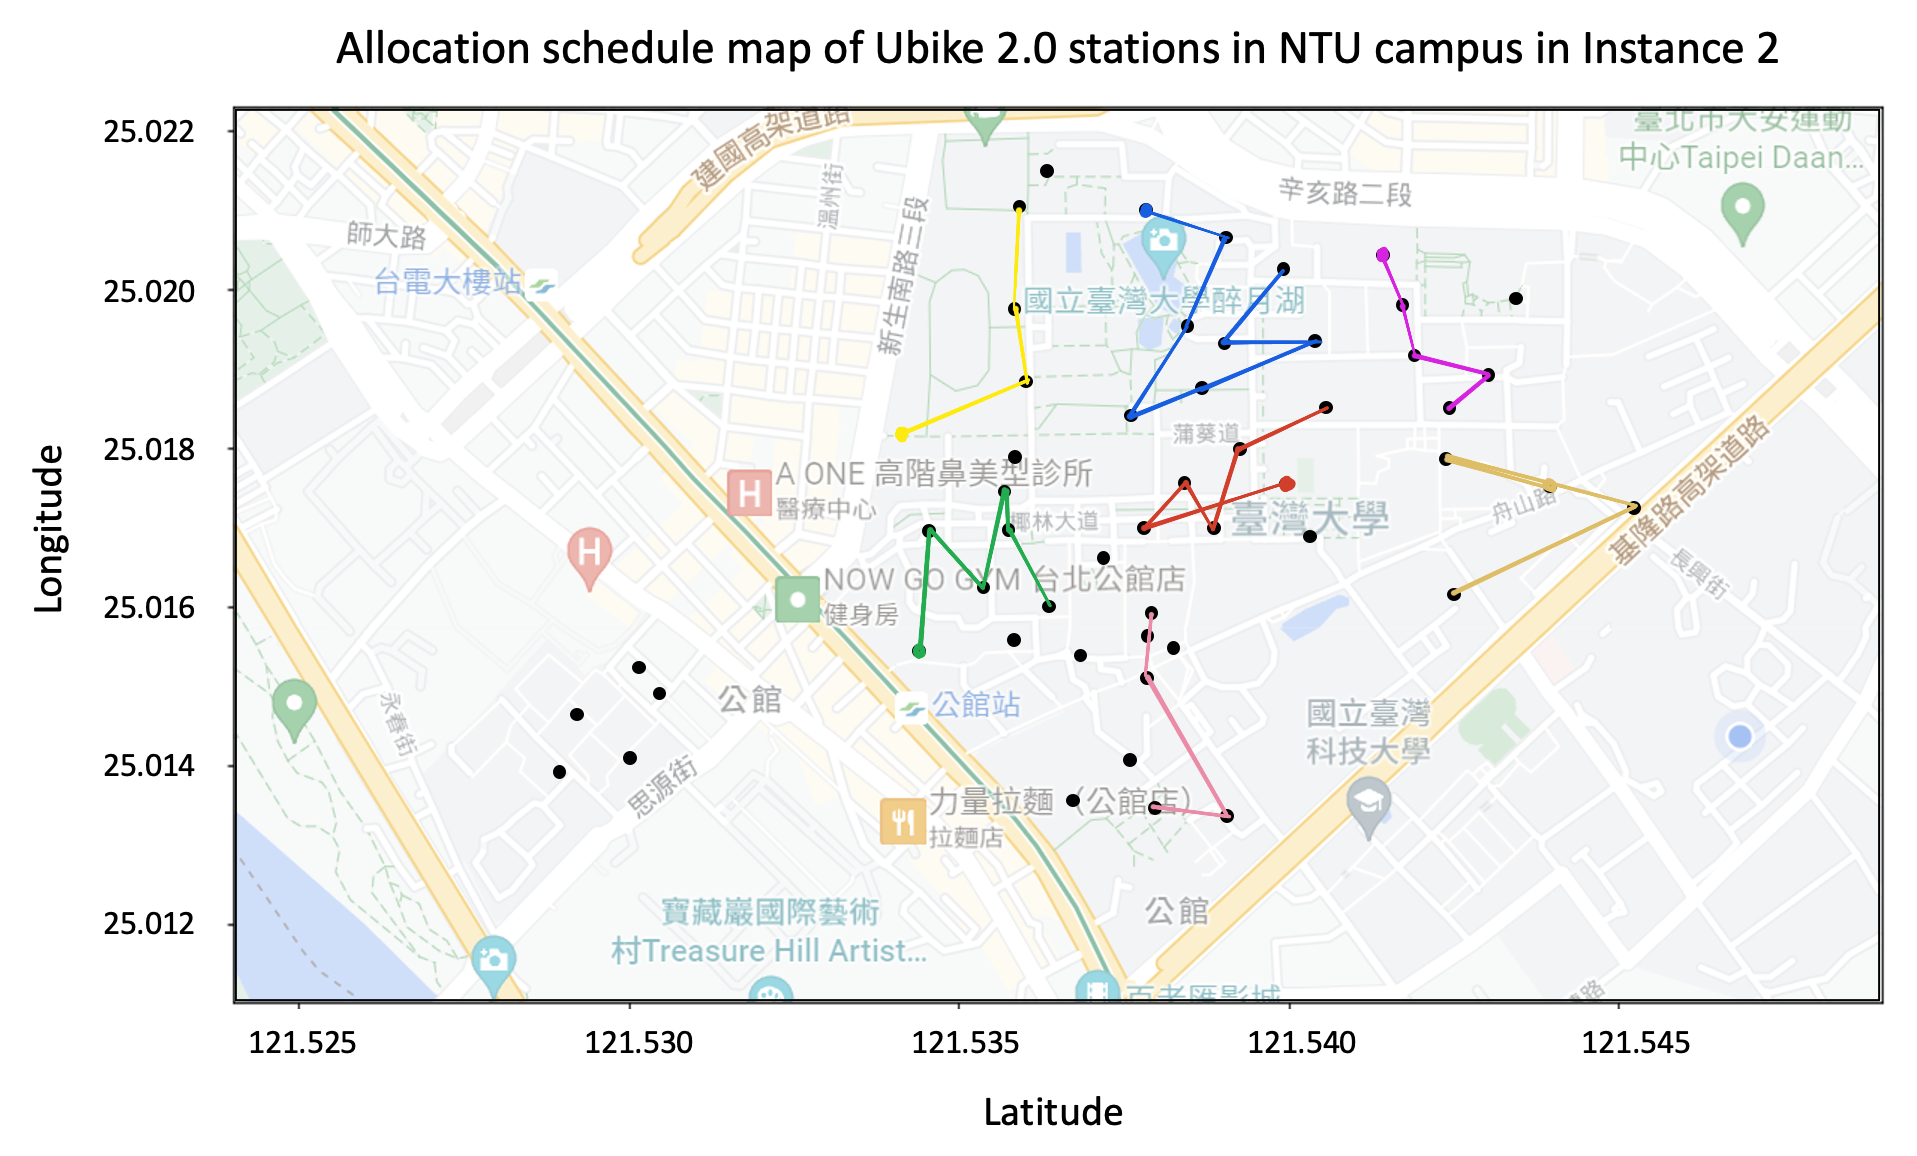
\includegraphics[width=0.9\textwidth]{Final/fig/Map2.png}
    \caption{The Allocation Schedule Map in Instance 2}
    \label{fig:2-map}
\end{figure}

\noindent Figure \ref{fig:2-map} depicts the routing map when k is equal to 8. Notice that one of the groups (the bottom-left one) does not need dispatching. Before the assignment (as shown in figure \ref{fig:2-before}), we may see that most of the stations are labeled in red, i.e., they are in shortages of bikes. Even though the assignment is completed (as shown in figure \ref{fig:2-after}), the red spots are not all eliminated; there are still some of them existing. \\

\noindent Our inference is that the number of bikes in this certain time is not as much as usual, so even more trucks are assigned in dispatching, perfect distribution of bikes is still cannot be achieved.

\begin{figure}[hbt]
\centering
	\begin{minipage}[b]{0.45\textwidth}
		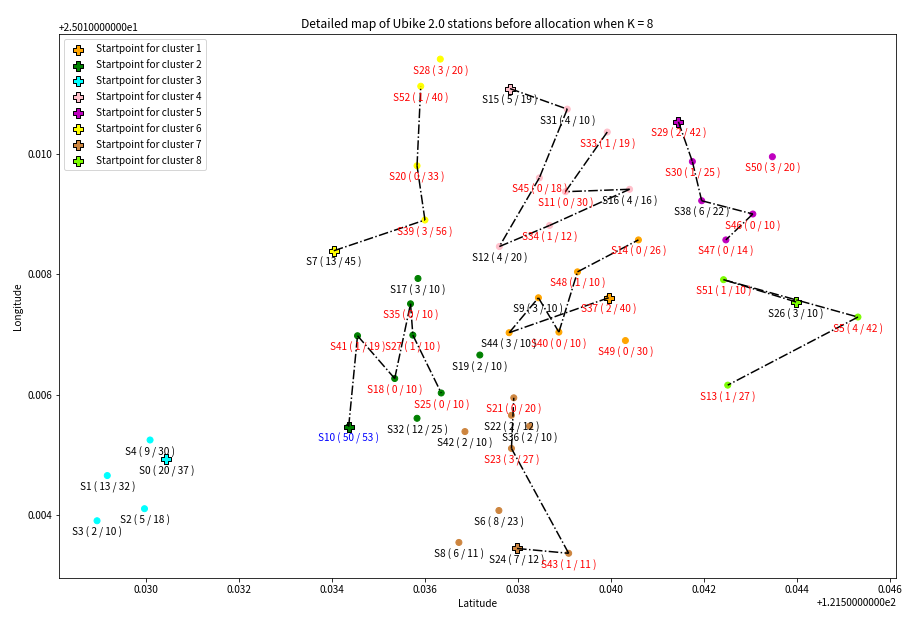
\includegraphics[width=\textwidth]{Final/fig/c2/4-8-4_Before Allocation Map.png}
		\caption{Detailed Ratio of YouBike Before Allocation in Instance 2}
		\label{fig:2-before}
	\end{minipage}
	\begin{minipage}[b]{0.05\textwidth}
		\quad
	\end{minipage}	
	\begin{minipage}[b]{0.45\textwidth}
		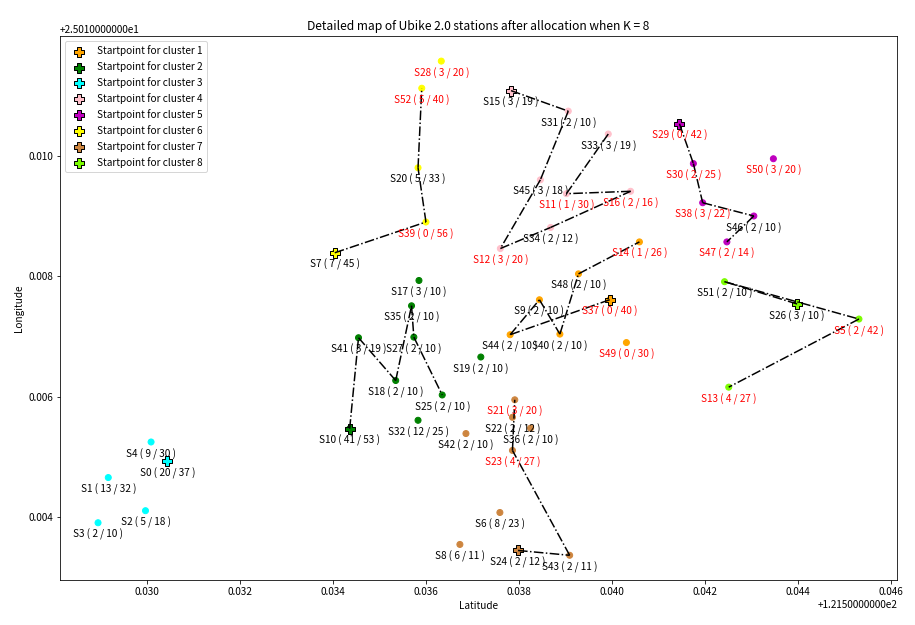
\includegraphics[width=\textwidth]{Final/fig/c2/4-8-3_After Allocation Map.png}
		\caption{Detailed Ratio of YouBike After Allocation in Instance 2}
		\label{fig:2-after}
	\end{minipage}
\end{figure}




% 值得一提的是,lambda越大表示此項決策越能包容站點出現缺車、或是較多車的狀態。而在限制較寬鬆的情形下,需要調度的站點與車輛數相對較少,這也是為什麼在instance 1(圖二) 與instance 2(圖六)中,都出現lambda越高成本越低的趨勢。

% 因此較好的決策應該不是一昧地選擇較低成本的方案,而是在成本預算的上限內,盡可能選擇lamba越小的方案作為調度方針。

\noindent What is worth mentioning is that larger $\lambda$ implies larger interval size of acceptable parking ratio, which means that the restriction in parking ratio is "looser", and hence fewer bikes need to be dispatched. That is why in both instance 1 and 2, higher $\lambda$ implies lower cost.\\ 

\noindent Therefore, to make a better decision is not focusing on picking out plans with lower cost adamantly. Choosing smaller $\lambda$ under a certain budget constraint is a more flexible way.



% \subsection{Instance 3: 6/3 10:00}

% Luckily, the incredible gurobi solver solved the instance 3.

% \begin{figure}[hbt]
%     \centering
%     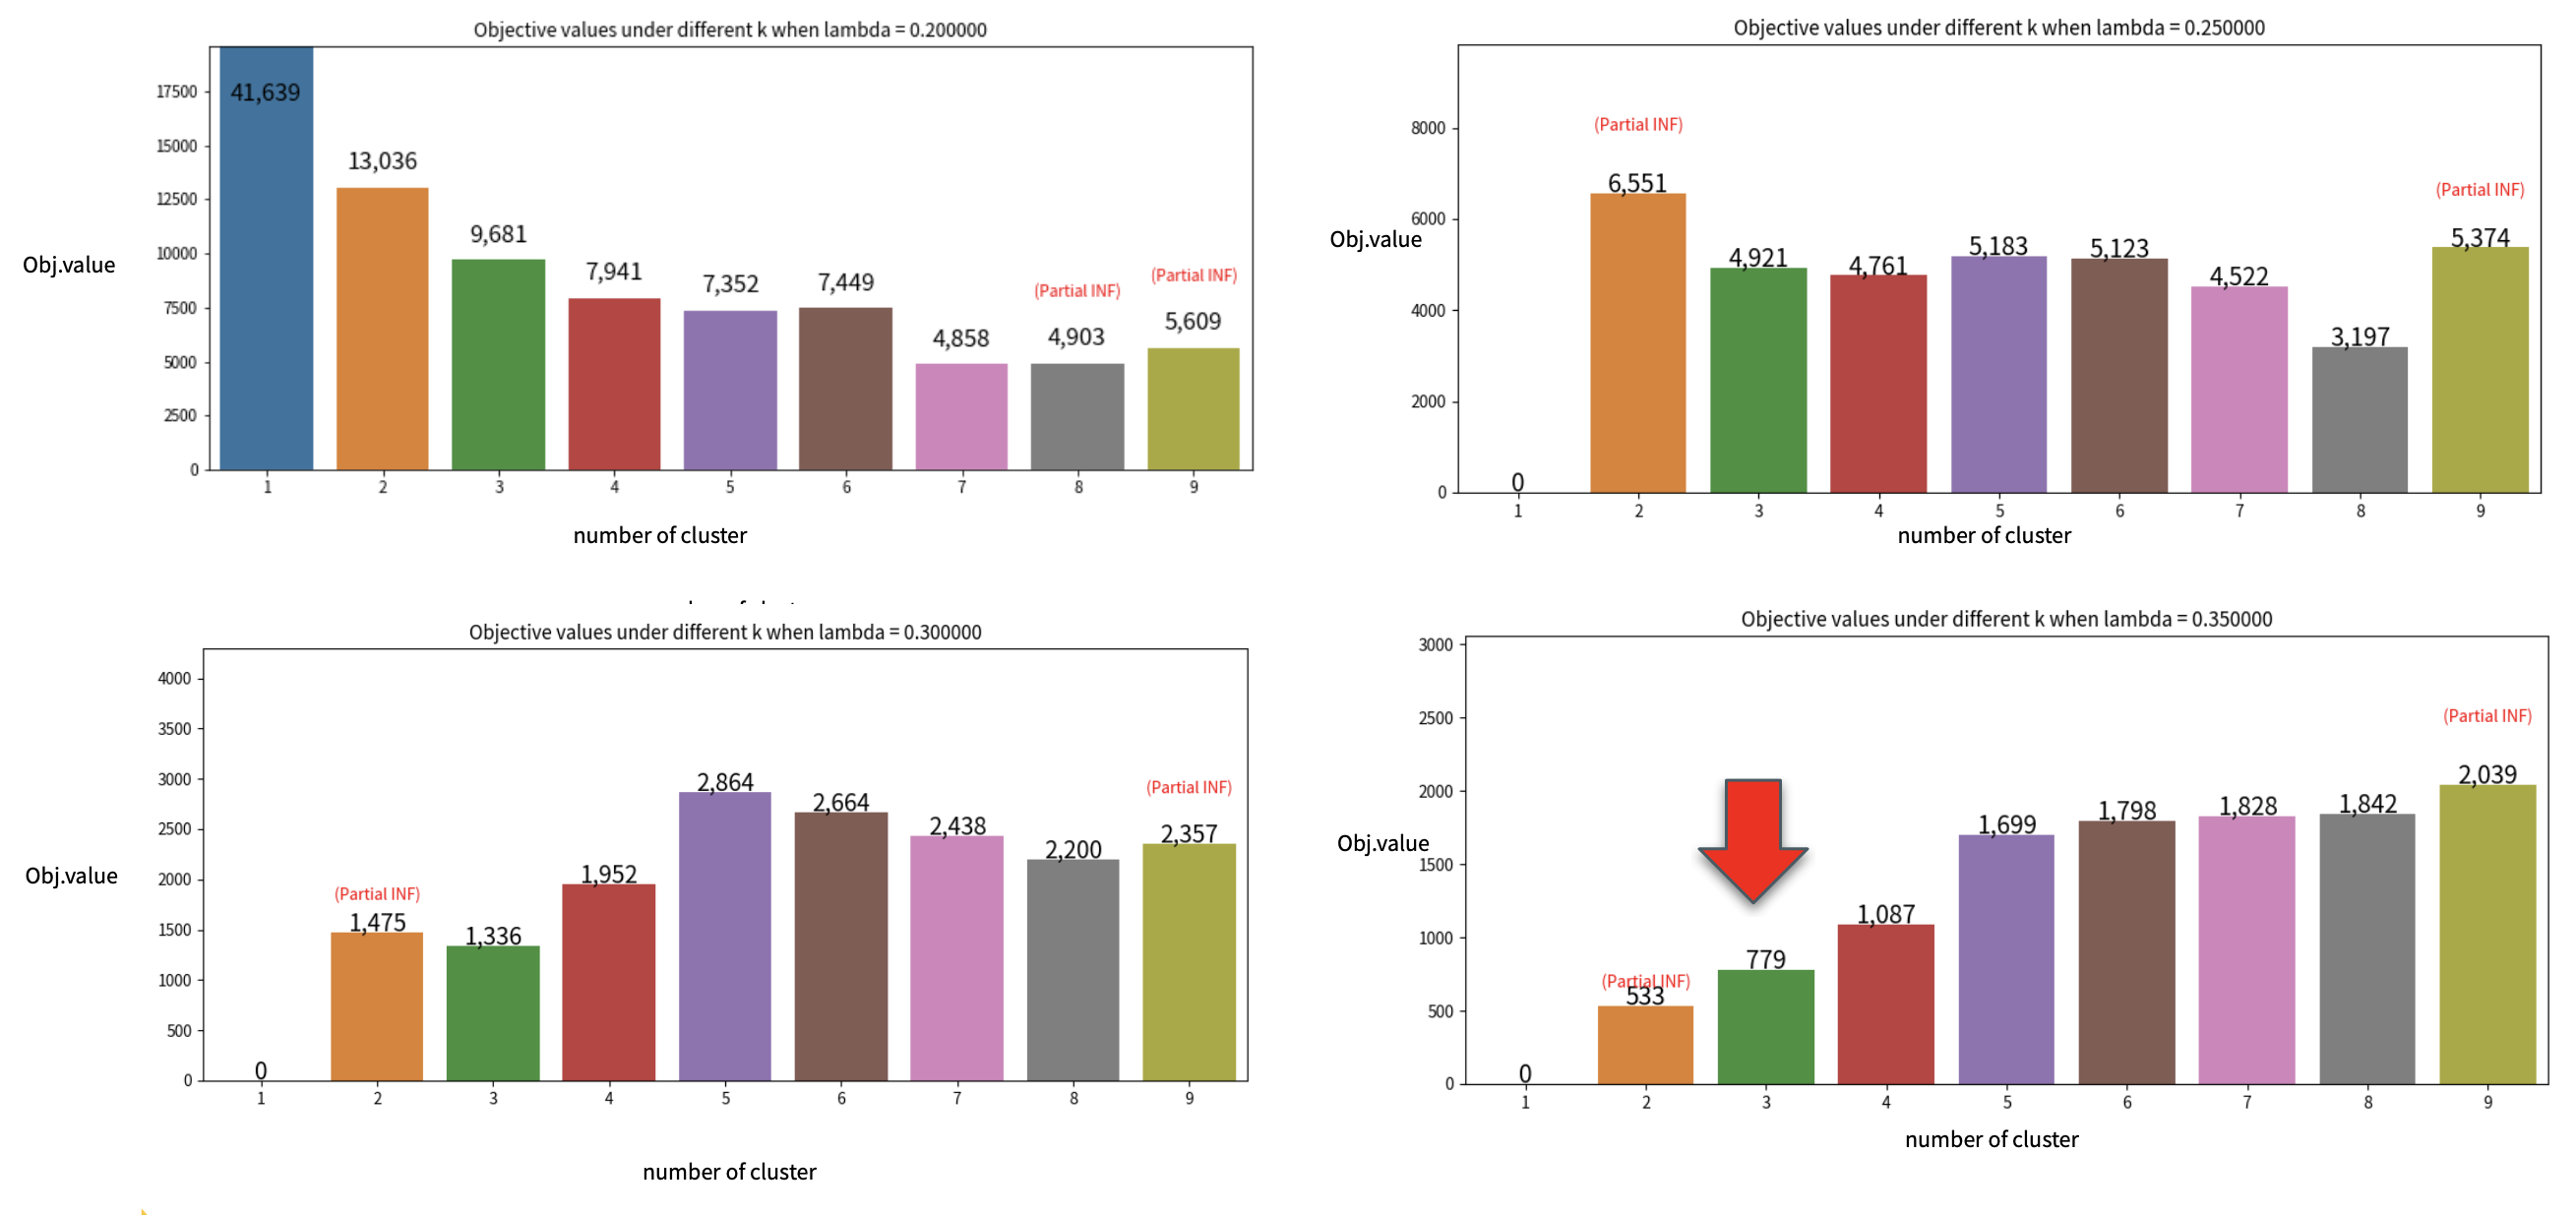
\includegraphics[width=0.9\textwidth]{Final/fig/bar_3.png}
%     \caption{Different $\lambda$ in Instance 3}
%     \label{fig:bar-3}
% \end{figure}

% \begin{figure}[hbt]
%     \centering
%     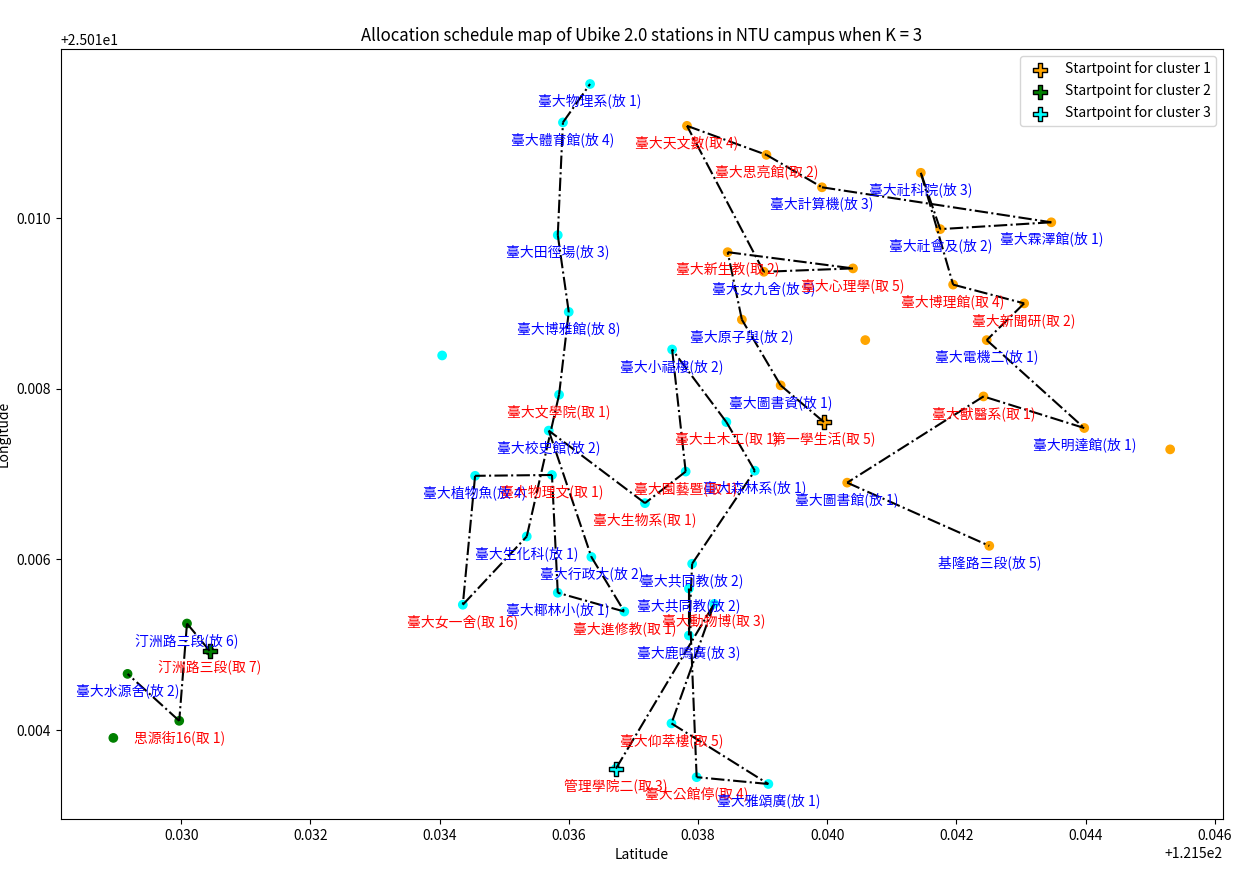
\includegraphics[width=0.7\textwidth]{Final/fig/c3/4-3-1_Allocation Schedule Map.png}
%     \caption{The allocation schedule map in Instance 3}
%     \label{fig:3-map}
% \end{figure}

% \begin{figure}[hbt]
% \centering
% 	\begin{minipage}[b]{0.45\textwidth}
% 		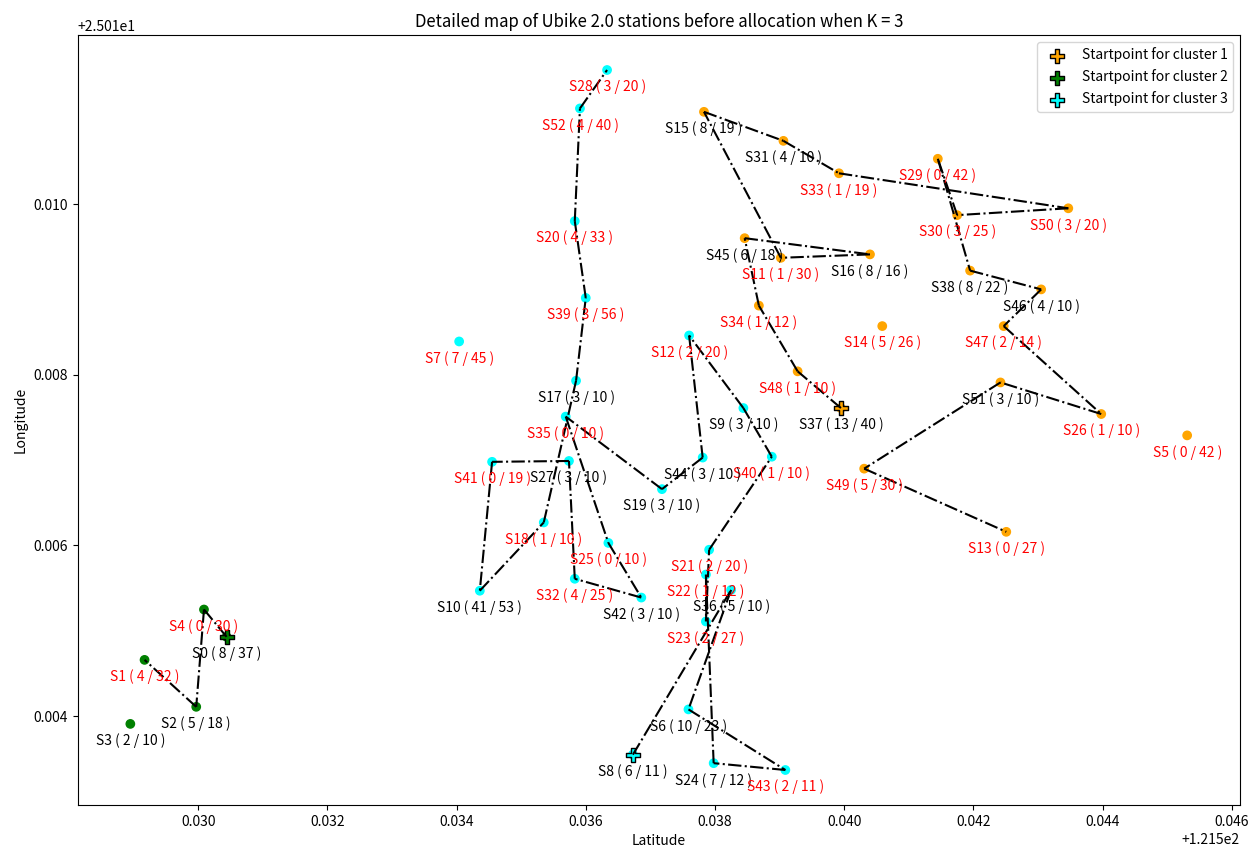
\includegraphics[width=\textwidth]{Final/fig/c3/4-3-4_Before Allocation Map.png}
% 		\caption{Detailed ratio of Ubike before allocation in Instance 3}
% 		\label{fig:3-before}
% 	\end{minipage}
% 	\begin{minipage}[b]{0.05\textwidth}
% 		\quad
% 	\end{minipage}	
% 	\begin{minipage}[b]{0.45\textwidth}
% 		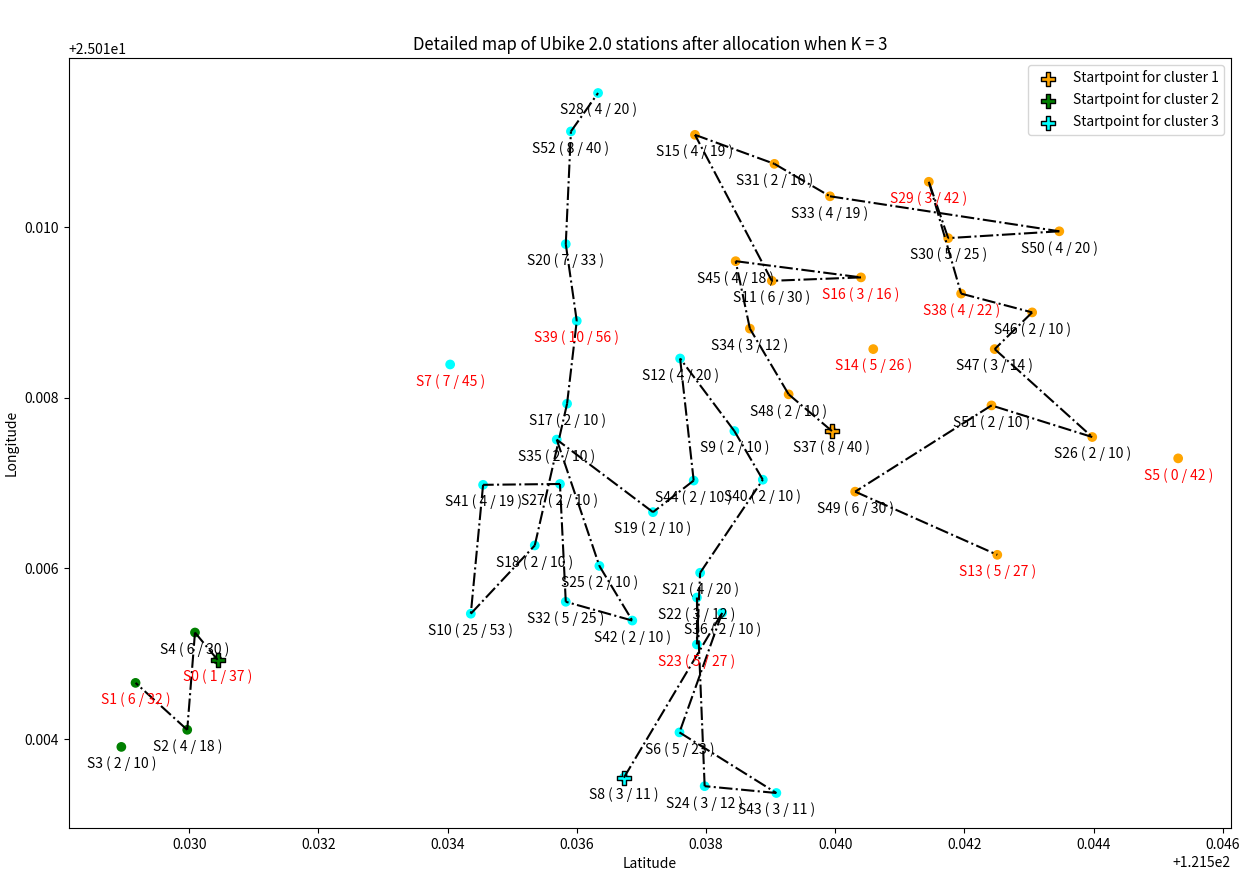
\includegraphics[width=\textwidth]{Final/fig/c3/4-3-3_After Allocation Map.png}
% 		\caption{Detailed ratio of Ubike after allocation in Instance 3}
% 		\label{fig:3-after}
% 	\end{minipage}
% \end{figure}

% \newpage
\section{Conclusions and Future Works}

\subsection{Conclusions}
As mentioned previously, at the end the system lists the results of different $(\lambda, k)$ and $\lambda$ can be decided according to the operator’s demand. For example, the four graphs in Figure 2 are all from instance 1 but with different $\lambda$s. If the operator choose smaller $\lambda$, then the interval will be smaller. Therefore, it will be easier to violate the percentage constraint and increase the cost. On the other hand, if the operator choose larger $\lambda$, then the interval will become larger. The results might be the one whose situation cannot be improved significantly. In instance 1, the operator has to choose among 1274, 525 and 512. If there is enough budget, 1274 will always be recommended without a doubt. However, the operator usually needs to make a trade-off between cost and service. In summary, our system provides several suggestions, but the final decision still rests with the operator.

\subsection{Future Works}

\subsubsection{Having More Than One Truck for Each Cluster}
Because the process is dynamic, the number of clusters is not always the same. For example, in previous hour $k$ is $4$ while in this hour $k$ is $2$, then the rest of the two trucks can support other areas. In that case, a single cluster can have more than one truck.

\subsubsection{Adding the Function for Data Collecting}
As mentioned previously, the final decision still rests with the operator, although data collection is not in the field of operations research. However, by doing so, this system could assist the operator in a more comprehensive way.

\subsubsection{Predicting the Demand Distribution for Next Period}
So far, what we are doing is minimizing the imbalance already happened. In the next step, we can try to predict when the next peak time will be and what the demand distribution is by then. By doing so, we can reposition the YouBikes or move the redundant trucks for backup in advance.

\end{document}




\section{Results}
A lot of instances are included in our analysis, and two of them are proposed to demonstrate the results of our assignment plan.

\subsection{Instance 1: 6/1 17:00}

\begin{figure}[hbt]
    \centering
    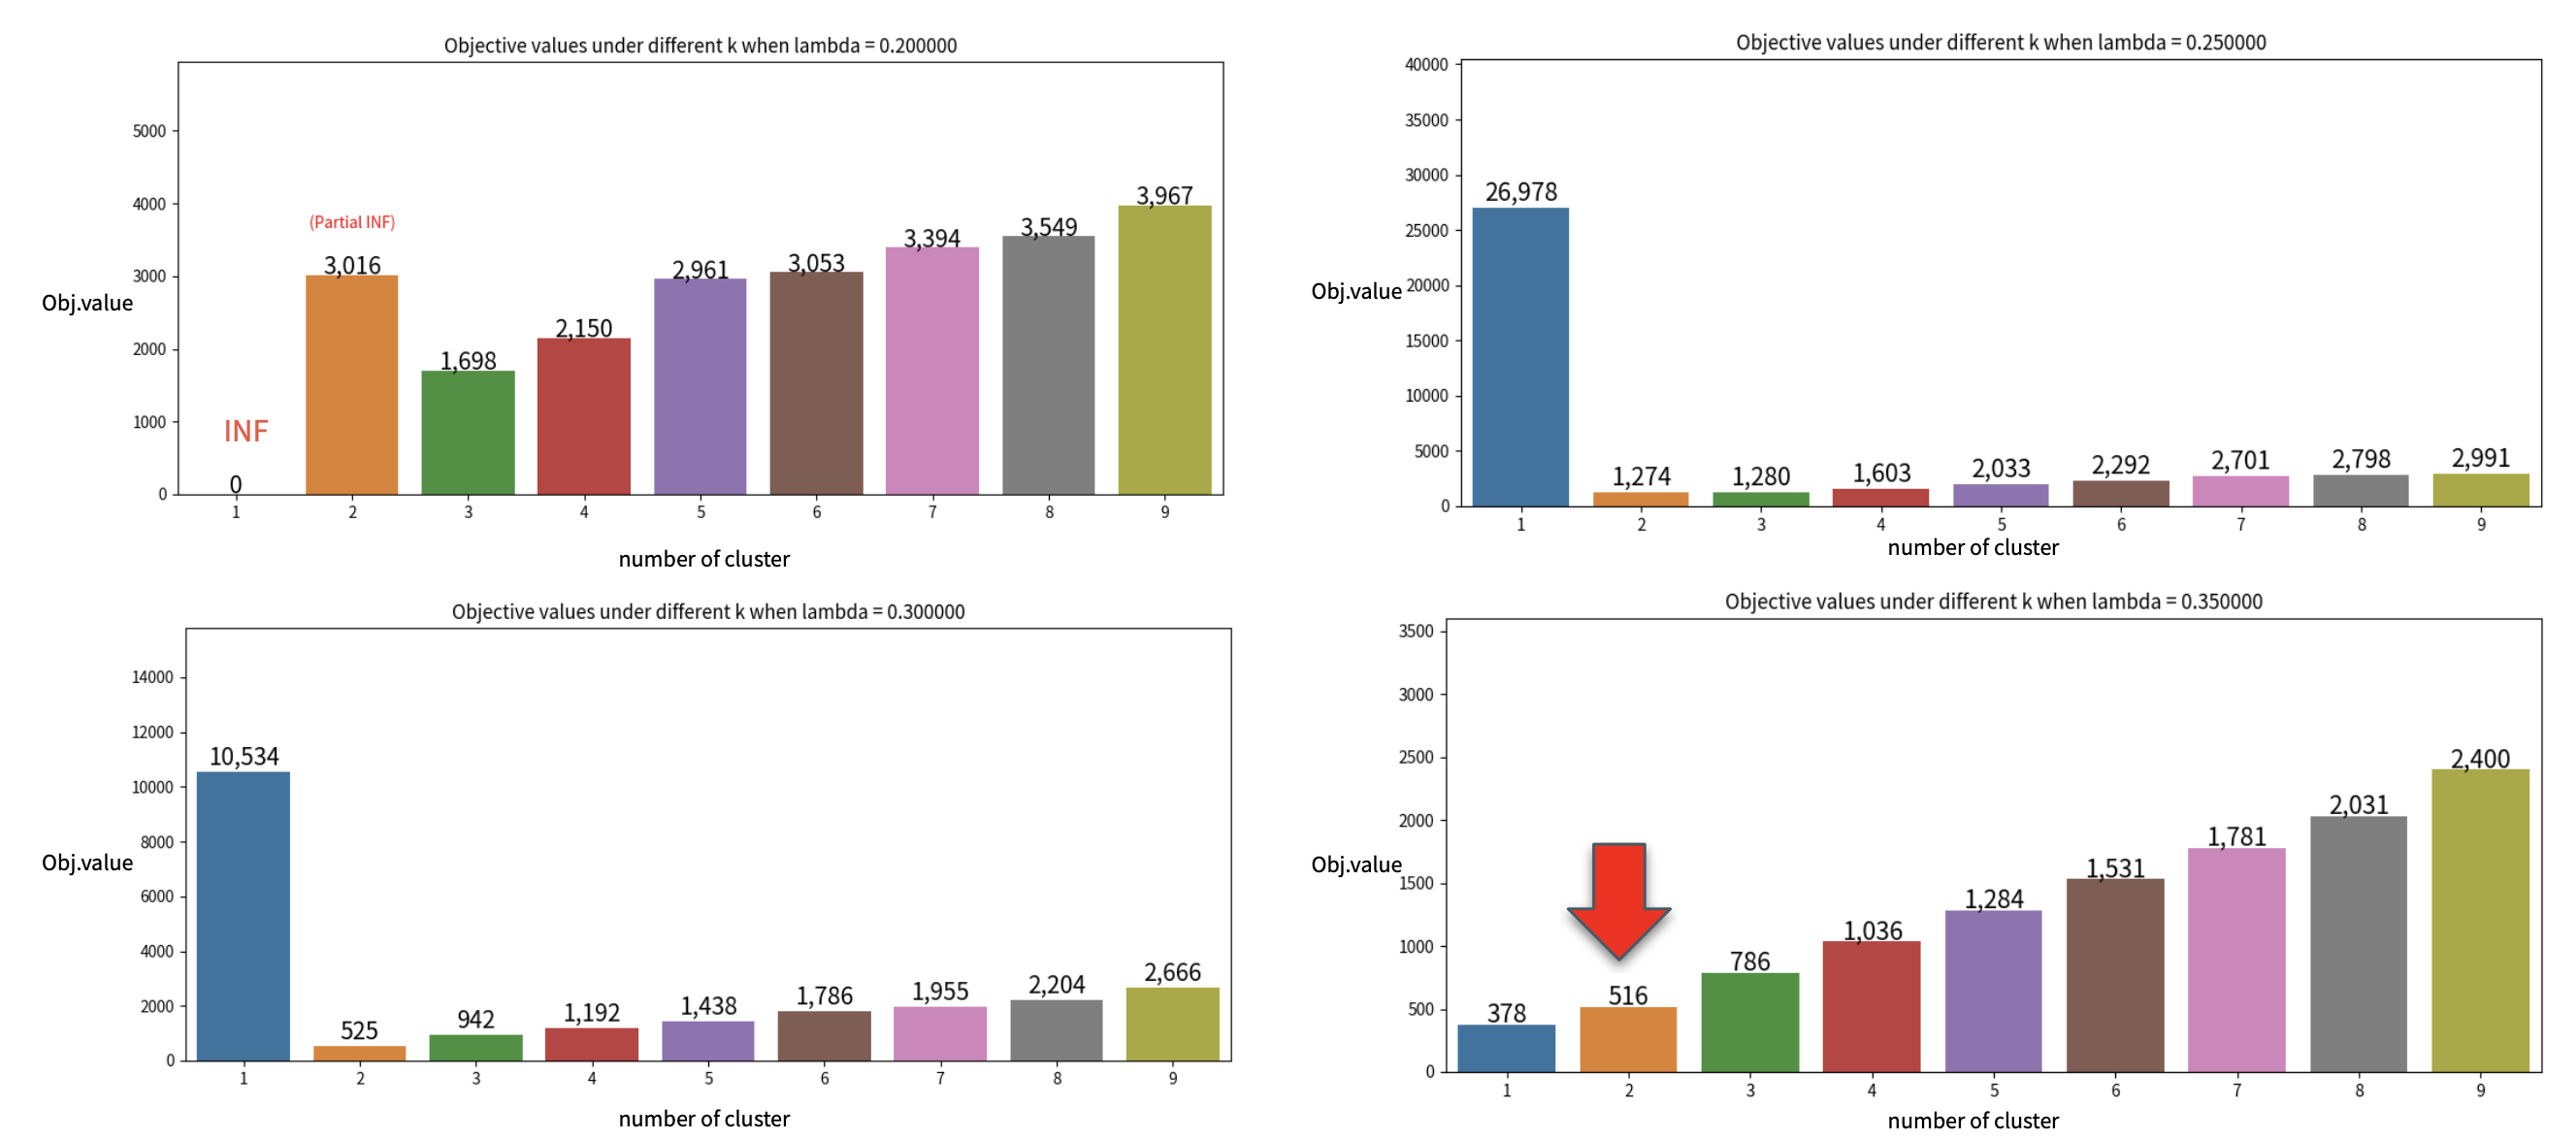
\includegraphics[width=0.9\textwidth]{Final/fig/bar_1.png}
    \caption{Objective Values under Different $\lambda$s and Clusters in Instance 1}
    \label{fig:bar-1}
\end{figure}


\noindent As one may see from figure \ref{fig:bar-1}, different combinations of $\lambda$s and $k$s are implemented. ($k^*, \lambda^*$) that leads to the least objective value would be selected as the value of the parameters. Note that some of them might be infeasible, and thus will not considered as one of the pairs of the parameter values.\\

In this case, $\lambda = 0.35$ and $k = 2$ works best among all the models.
\begin{figure}[hbt]
    \centering
    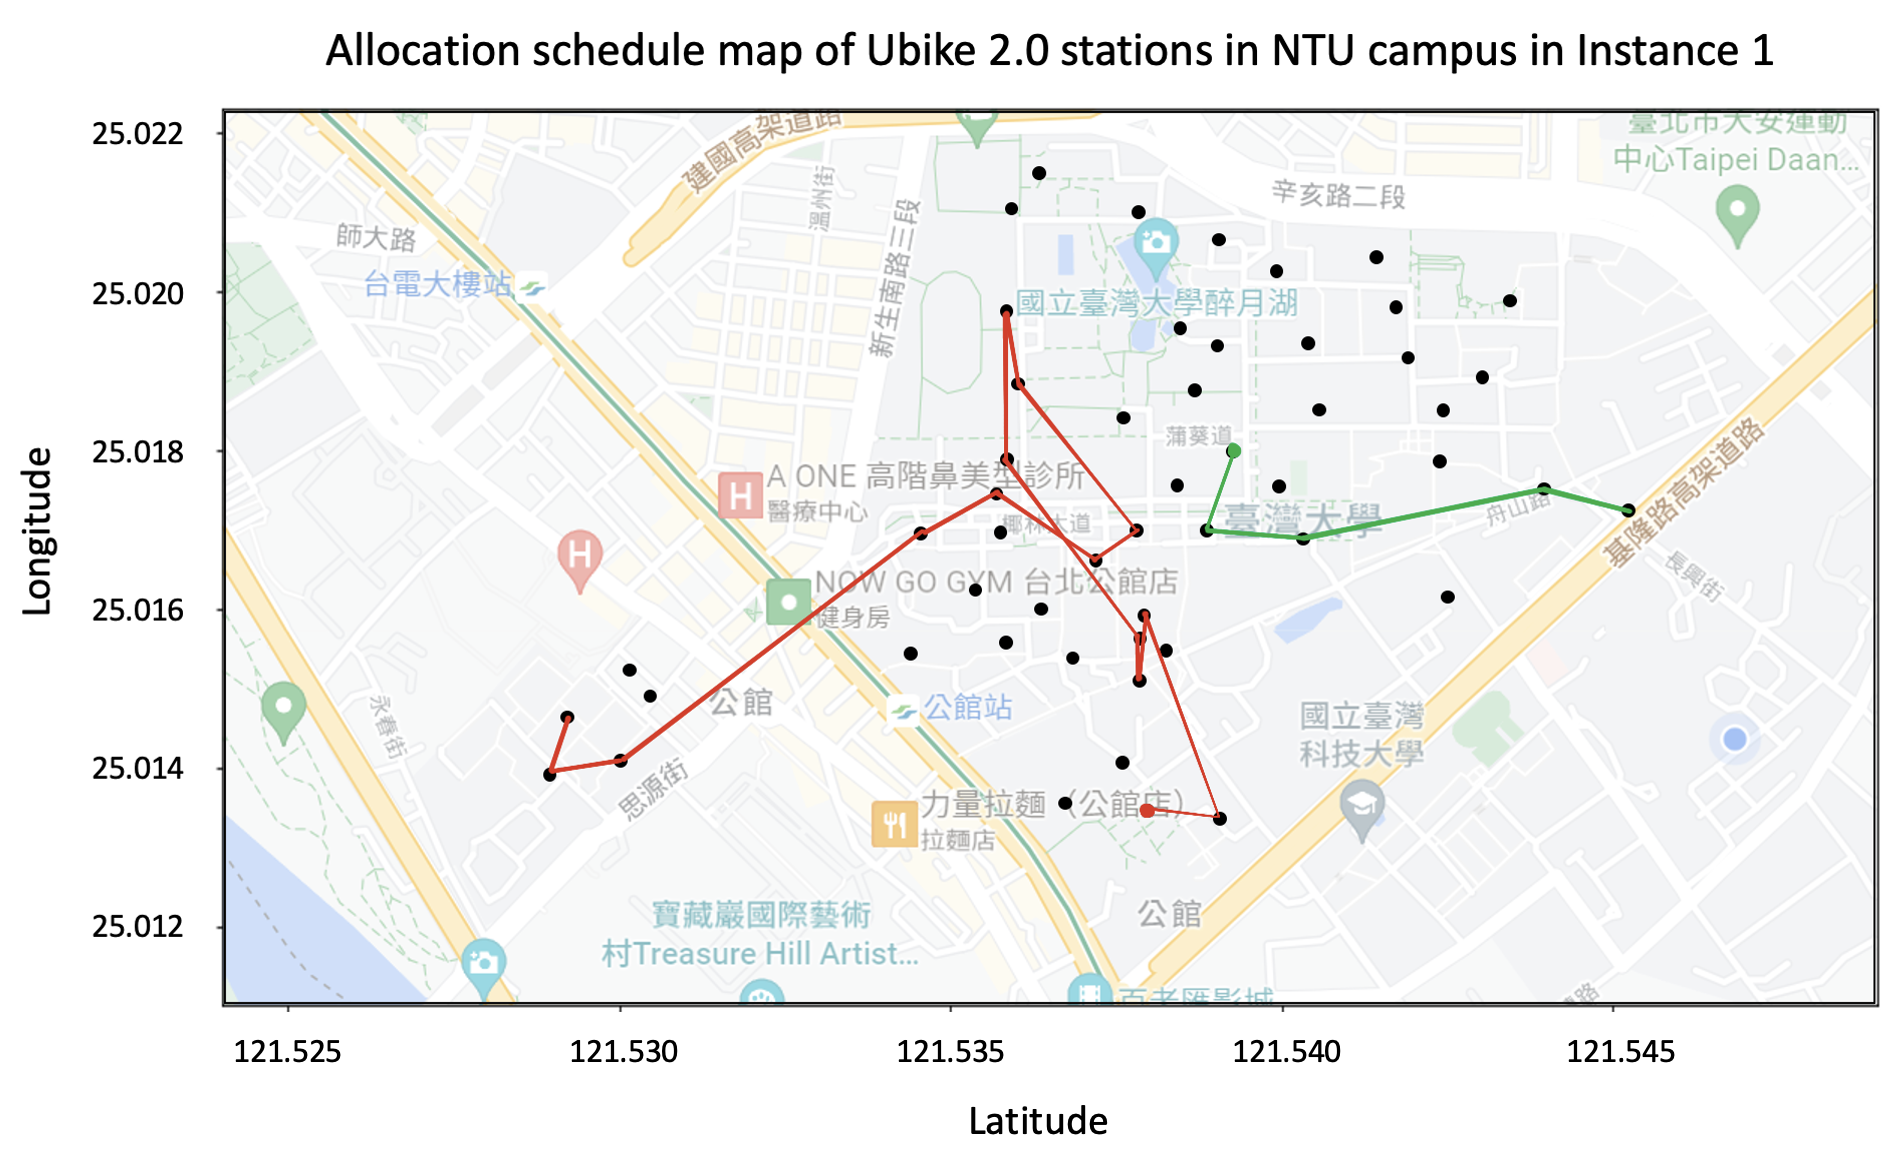
\includegraphics[width=0.8\textwidth]{Final/fig/Map1.png}
    \caption{The Allocation Schedule Map in Instance 1}
    \label{fig:1-map}
\end{figure}


\noindent Figure \ref{fig:1-map} shows the allocation schedule map, stations labelled in blue are the ones whose parking rate exceeds the upper bound and stations labelled in red are the ones whose parking rate falls beneath the lower bound. In the following trial, our goal is to dispatch bikes to the red stations by taking bikes from the blue ones. By doing so, the number of bikes in each stations are expected to be balanced. \\

\noindent Before any bike assignment, either stations labelled in red or stations labelled in blue indicate that there are imbalanced bike distribution among different locations. To evaluate our program, a comparison is adopted as shown in figure \ref{fig:1-before} and \ref{fig:1-after}. After our implementation, one might be amazed that only 4 stations are having parking rate out of acceptable range. It seems that our implementation quite outperforms.






\begin{figure}[hbt]
\centering
	\begin{minipage}[b]{0.45\textwidth}
		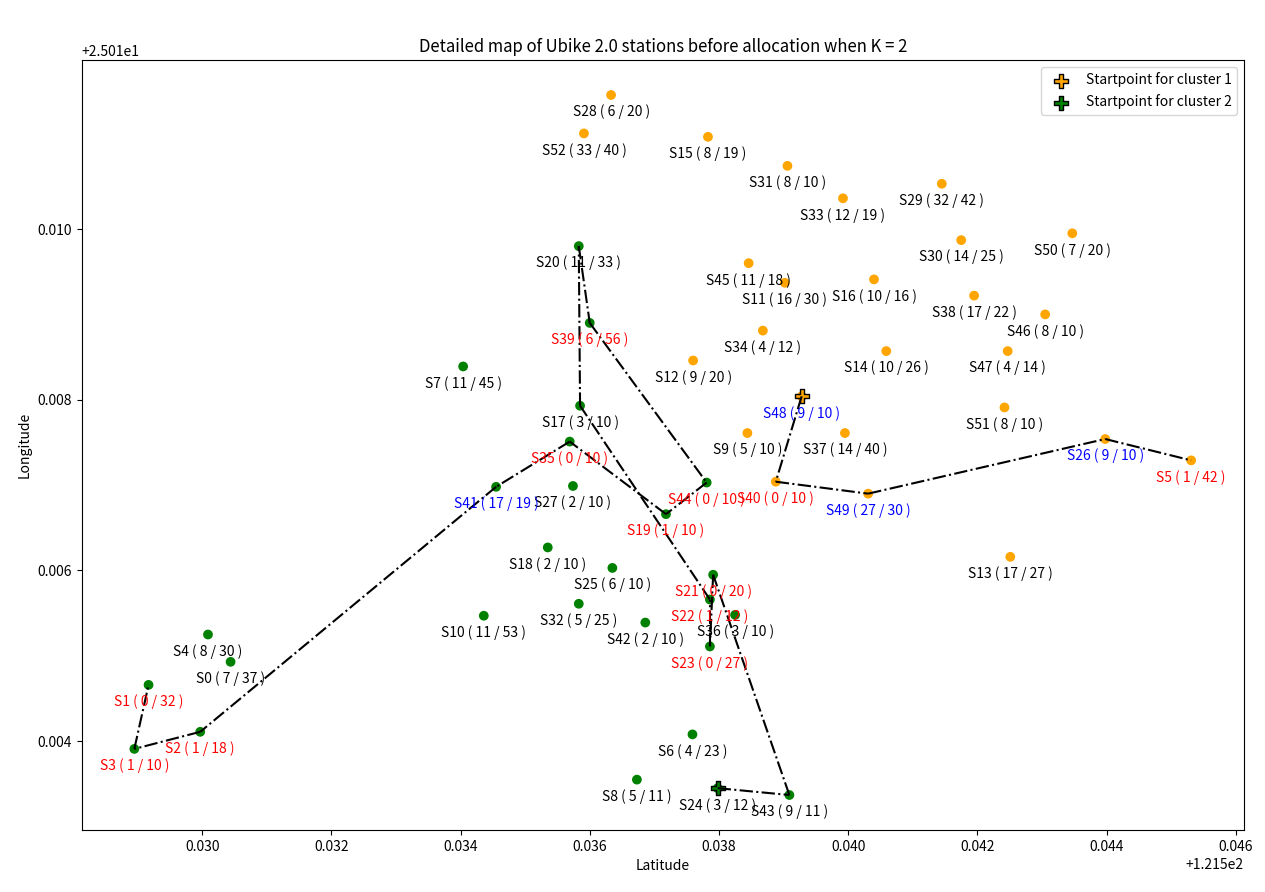
\includegraphics[width=\textwidth]{Final/fig/c1/4-2-4_Before Allocation Map.png}
		\caption{Detailed Ratio of YouBike Before Allocation in Instance 1}
		\label{fig:1-before}
	\end{minipage}
	\begin{minipage}[b]{0.05\textwidth}
		\quad
	\end{minipage}	
	\begin{minipage}[b]{0.45\textwidth}
		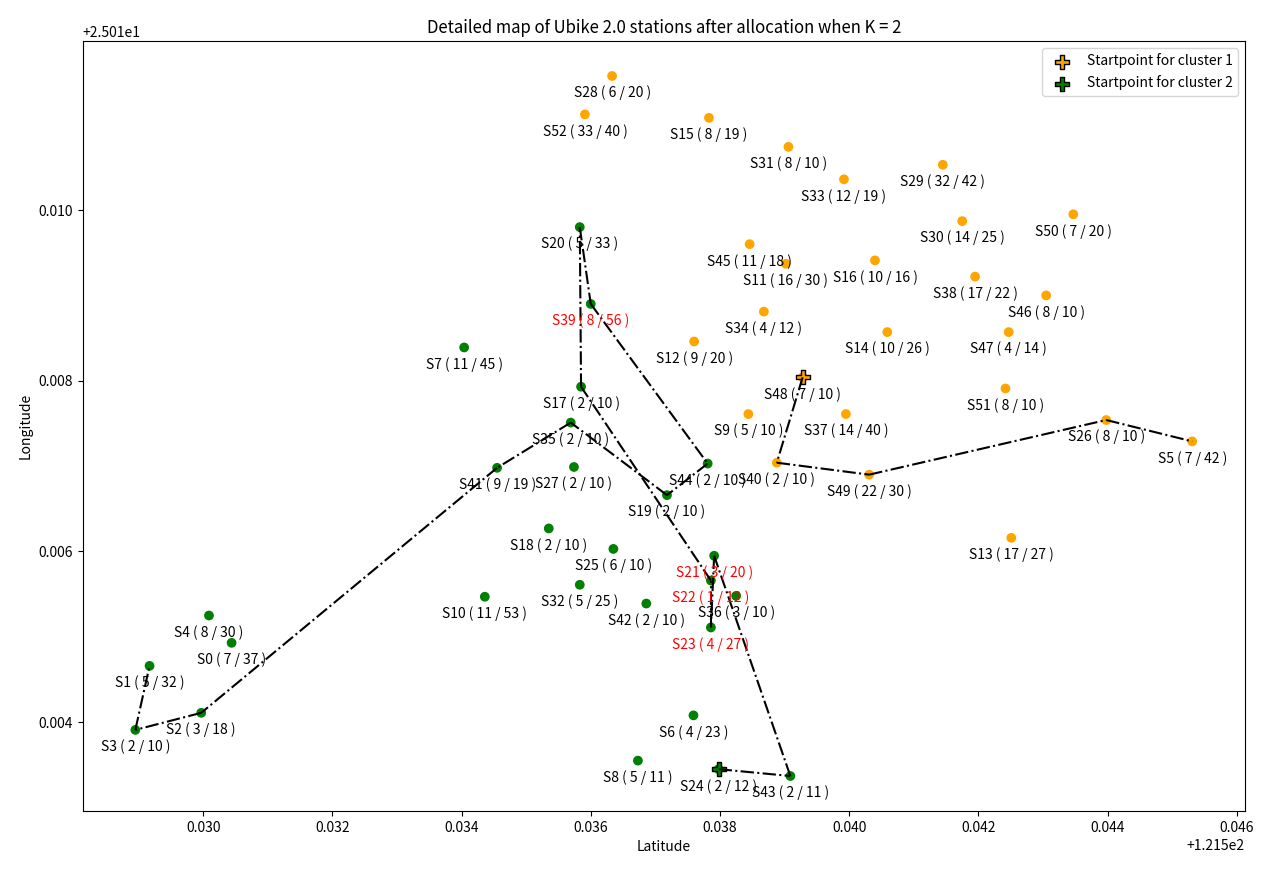
\includegraphics[width=\textwidth]{Final/fig/c1/4-2-3_After Allocation Map.png}
		\caption{Detailed Ratio of YouBike After Allocation in Instance 1}
		\label{fig:1-after}
	\end{minipage}
\end{figure}

\subsection{Instance 2: 6/3 8:00}

\begin{figure}[hbt]
    \centering
    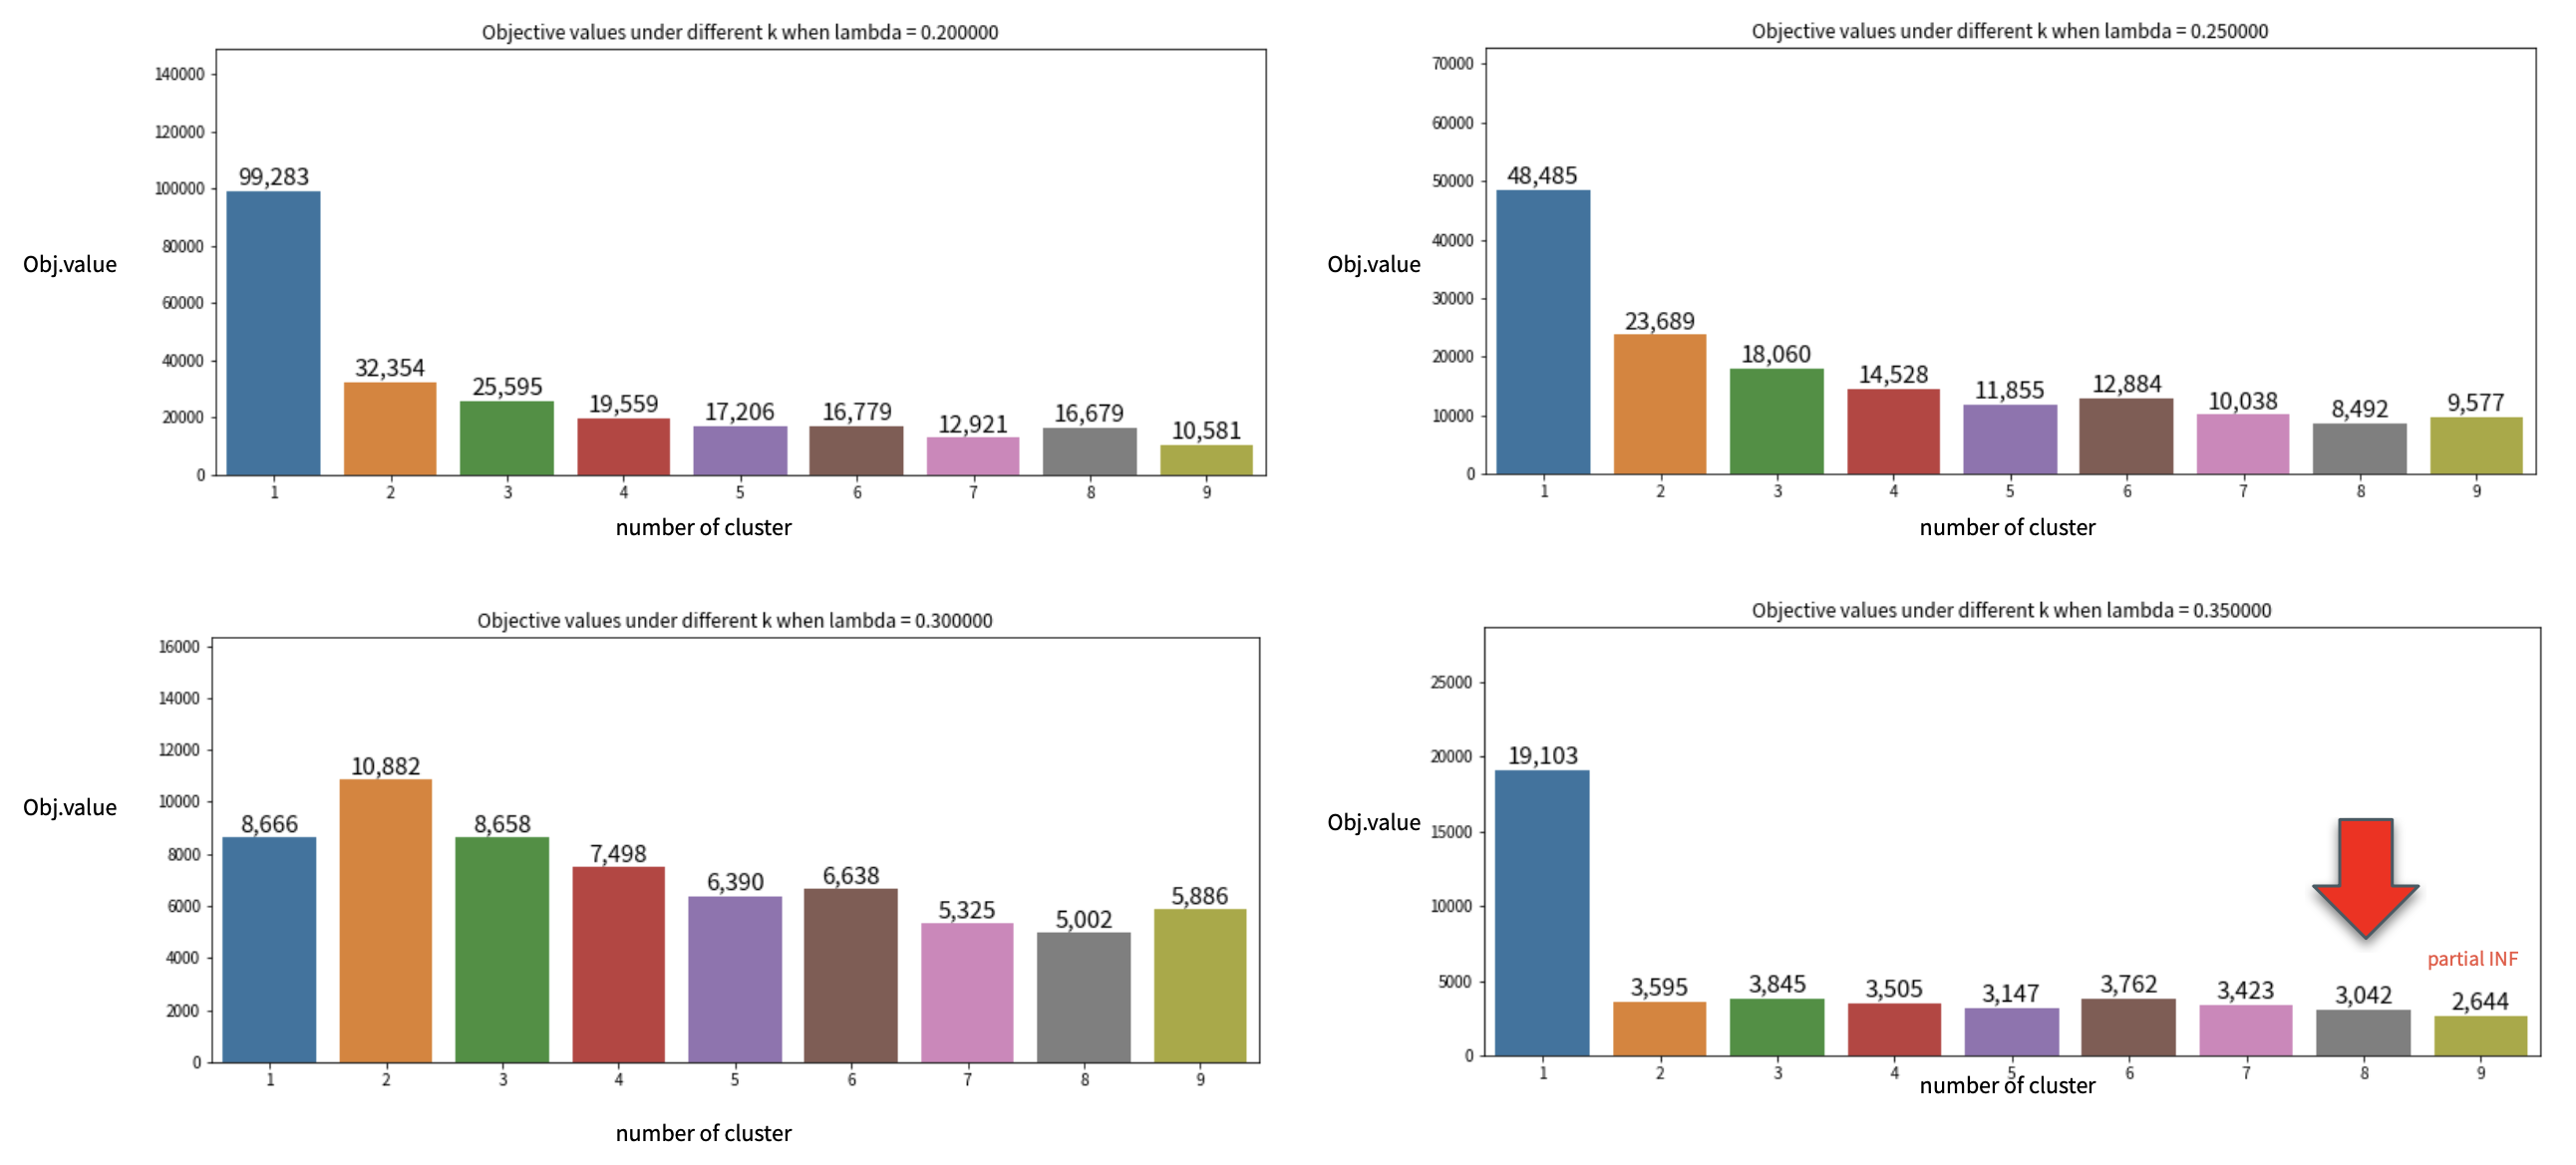
\includegraphics[width=0.9\textwidth]{Final/fig/bar_2.png}
    \caption{Objective Values under Different $\lambda$s and Clusters in Instance 2}
    \label{fig:bar-2}
\end{figure}

\begin{figure}[hbt]
    \centering
    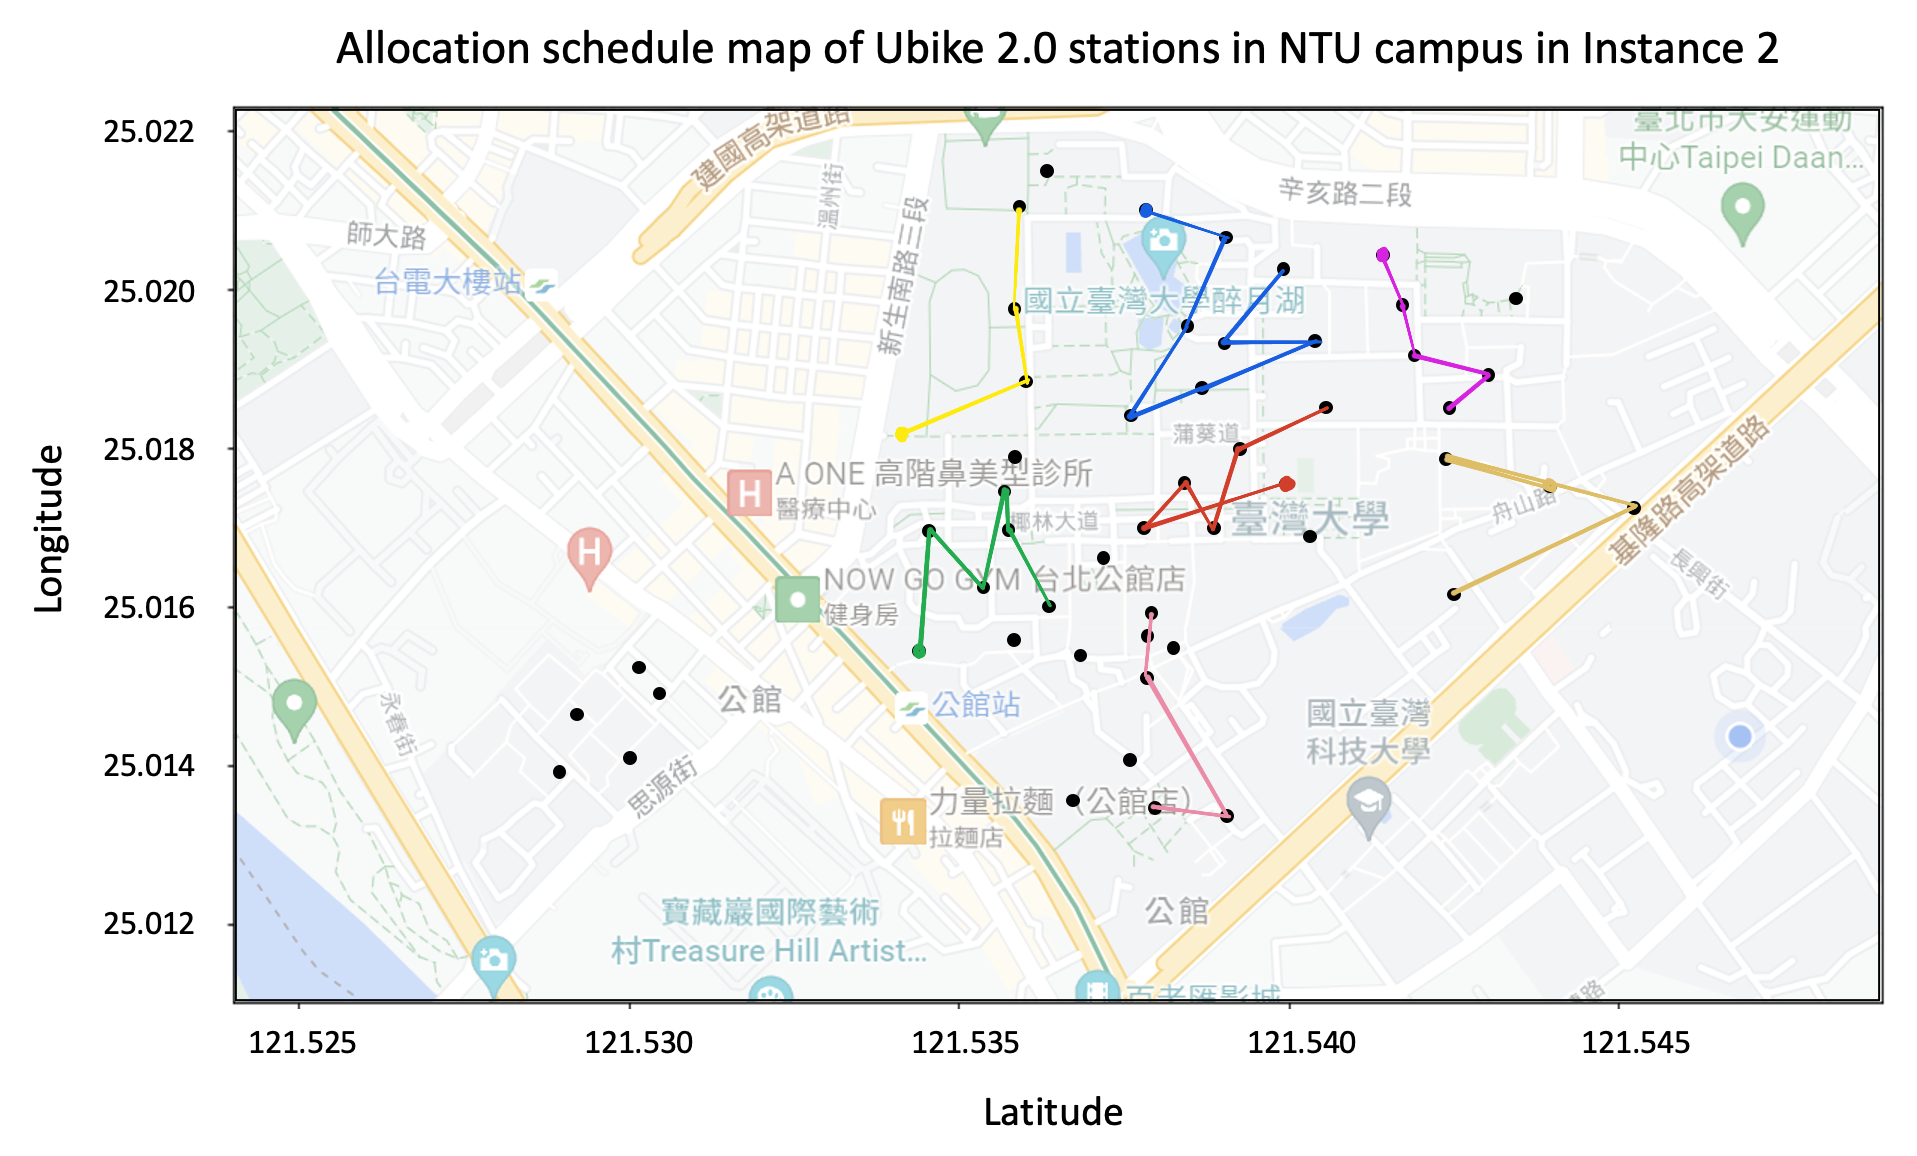
\includegraphics[width=0.8\textwidth]{Final/fig/Map2.png}
    \caption{The Allocation Schedule Map in Instance 2}
    \label{fig:2-map}
\end{figure}

\begin{figure}[hbt]
\centering
	\begin{minipage}[b]{0.45\textwidth}
		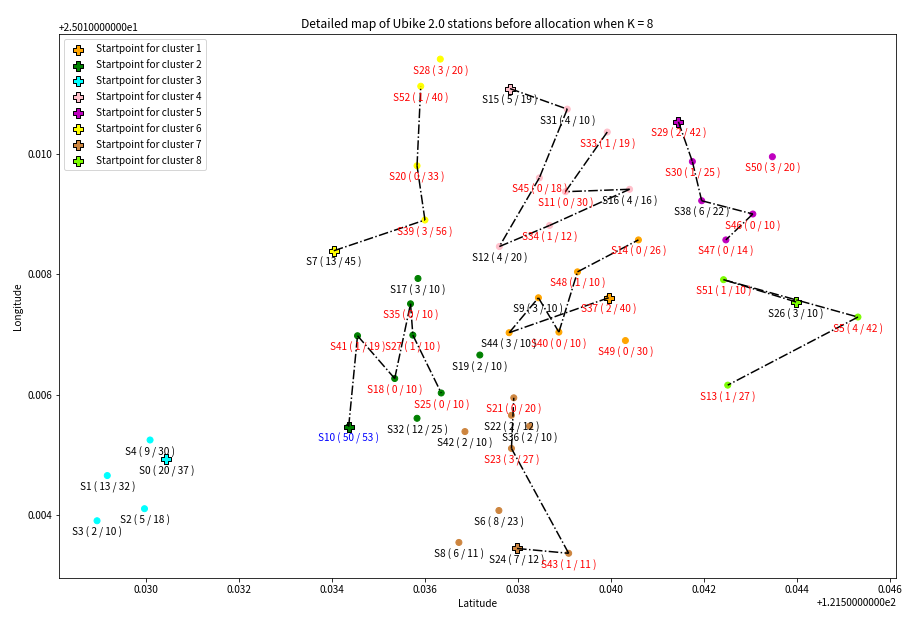
\includegraphics[width=\textwidth]{Final/fig/c2/4-8-4_Before Allocation Map.png}
		\caption{Detailed Ratio of YouBike Before Allocation in Instance 2}
		\label{fig:2-before}
	\end{minipage}
	\begin{minipage}[b]{0.05\textwidth}
		\quad
	\end{minipage}	
	\begin{minipage}[b]{0.45\textwidth}
		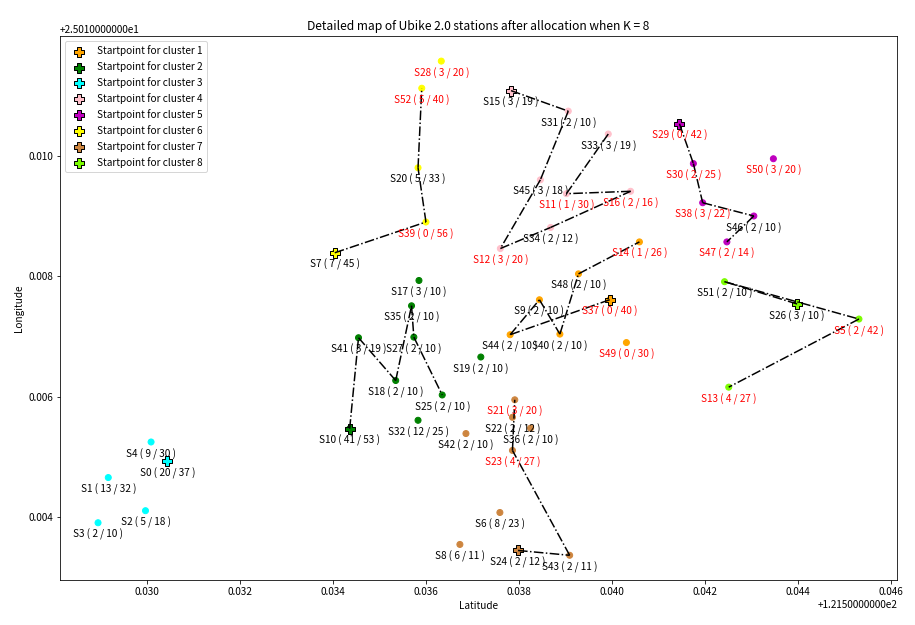
\includegraphics[width=\textwidth]{Final/fig/c2/4-8-3_After Allocation Map.png}
		\caption{Detailed Ratio of YouBike After Allocation in Instance 2}
		\label{fig:2-after}
	\end{minipage}
\end{figure}

\noindent As figure \ref{fig:bar-2} shows, the optimal $\lambda$ is $0.35$ and the optimal $k$ is $8$.\\
It is observed that jobs in 8 trucks cannot be done easily without having a large bike flow, which shows that the number of bikes in this time slot is quite imbalanced among YouBike stations. Figure \ref{fig:2-before} demonstrates that there are only few bikes in each station.\\
Despite the fact that all bikes in NTU area are dispatched, one may see that there are still red stations, which cannot be neglected, indicating lack of available bikes. However, figure \ref{fig:2-after} shows around 40\% of stations are dispatched with bikes and their acceptable parking ratios are achieved.